%% 
%% Copyright 2007-2019 Elsevier Ltd
%% 
%% This file is part of the 'Elsarticle Bundle'.
%% ---------------------------------------------
%% 
%% It may be distributed under the conditions of the LaTeX Project Public
%% License, either version 1.2 of this license or (at your option) any
%% later version.  The latest version of this license is in
%%    http://www.latex-project.org/lppl.txt
%% and version 1.2 or later is part of all distributions of LaTeX
%% version 1999/12/01 or later.
%% 
%% The list of all files belonging to the 'Elsarticle Bundle' is
%% given in the file `manifest.txt'.
%% 
%% Template article for Elsevier's document class `elsarticle'
%% with harvard style bibliographic references

%\documentclass[preprint,12pt,authoryear]{elsarticle}

%% Use the option review to obtain double line spacing
\documentclass[authoryear,preprint,review,12pt]{elsarticle}

%% Use the options 1p,twocolumn; 3p; 3p,twocolumn; 5p; or 5p,twocolumn
%% for a journal layout:
%% \documentclass[final,1p,times,authoryear]{elsarticle}
%% \documentclass[final,1p,times,twocolumn,authoryear]{elsarticle}
%% \documentclass[final,3p,times,authoryear]{elsarticle}
%% \documentclass[final,3p,times,twocolumn,authoryear]{elsarticle}
%% \documentclass[final,5p,times,authoryear]{elsarticle}
%% \documentclass[final,5p,times,twocolumn,authoryear]{elsarticle}

%% For including figures, graphicx.sty has been loaded in
%% elsarticle.cls. If you prefer to use the old commands
%% please give \usepackage{epsfig}

%% The amssymb package provides various useful mathematical symbols
\usepackage{amssymb}
%% The amsthm package provides extended theorem environments
%% \usepackage{amsthm}

\usepackage{siunitx}  % for degree celsius
\usepackage{multirow} % for the table
\usepackage{booktabs} % fot toprule, midrule
\usepackage{longtable}

\usepackage{color,soul} % highlight 

%% change caption of figure name
%\renewcommand{\figurename}{Fig.}
% or 
%\usepackage[figurename=Fig.]{caption}

% for track changes in revision version, comment this one if want the final version
%\usepackage{changes}
%\usepackage[final]{changes}

\usepackage{hyperref} %for breaking long url

%% The lineno packages adds line numbers. Start line numbering with
%% \begin{linenumbers}, end it with \end{linenumbers}. Or switch it on
%% for the whole article with \linenumbers.
%% \usepackage{lineno}

\usepackage{lineno}
\linenumbers

\journal{Remote Sensing of Environment}

\begin{document}

\begin{frontmatter}

%% Title, authors and addresses

%% use the tnoteref command within \title for footnotes;
%% use the tnotetext command for theassociated footnote;
%% use the fnref command within \author or \address for footnotes;
%% use the fntext command for theassociated footnote;
%% use the corref command within \author for corresponding author footnotes;
%% use the cortext command for theassociated footnote;
%% use the ead command for the email address,
%% and the form \ead[url] for the home page:
%% \title{Title\tnoteref{label1}}
%% \tnotetext[label1]{}
%% \author{Name\corref{cor1}\fnref{label2}}
%% \ead{email address}
%% \ead[url]{home page}
%% \fntext[label2]{}
%% \cortext[cor1]{}
%% \address{Address\fnref{label3}}
%% \fntext[label3]{}

%\ead{huanglingcao@link.cuhk.edu.hk}

\title{Automatically quantifying evolution of retrogressive thaw slumps in Beiluhe (Tibetan Plateau) from multi-temporal CubeSat images}

%\title{Mapping Retrogressive Thaw Slumps in the Beiluhe Region (Tibetan Plateau) from CubeSat Images using Deep Learning}

%% use optional labels to link authors explicitly to addresses:
%% \author[label1,label2]{}
%% \address[label1]{}
%% \address[label2]{}

\author[a]{Lingcao Huang}
\author[a]{Lin Liu}
\author[b]{more}
%\author[b]{Jing Luo}
%\author[b]{Zhanju Lin}
%\author[b]{Fujun Niu}



\address[a]{Earth System Science Programme, Faculty of Science, The Chinese University of Hong Kong, Hong Kong SAR, China.}
\address[b]{Add a few more co-authors?}
%\address[b]{Northwest Institute of Eco-Environment and Resources, Chinese Academy of Sciences, Lanzhou, China.}

\begin{abstract}

Retrogressive thaw slumps (RTSs) are among the most dynamic landforms resulting from the thawing of ice-rich permafrost. 
However, their distribution and evolution are poorly quantified because most of them scatter in remote and inaccessible permafrost areas. % due to the challenges in accurately mapping them from remote sensing images. 
In this study, we propose a method that integrates deep learning, change detection, and medial axis transform, aiming to automatically quantify the RTS development on multi-temporal images in the Beiluhe region from 2017 to 2019. 
The images are taken by the Planet CubeSat constellation with high spatial and temporal resolution.
The experiments show that automatic delineation based on deep learning can produce similar results to manual delineation, which is sufficient for quantifying the changes of RTS boundaries in different years. 
Our method reveals that among 342 RTSs in the Beiluhe region, 83\% and 76\% of them expanded from 2017 to 2018 and 2018 to 2019, respectively.
For the expansion from 2017 to 2018, the average and maximum expanding areas are 0.20 ha and 1.47 ha, while the average and maximum retreat distances are 21.3 m and 91 m, respectively;
the ones from 2018 to 2019 are 0.22 ha, 2.53 ha, 25.0 m, and 212 m, respectively. 
The results show that the method can quantify RTS development automatically on multi-temporal images and can be potentially applied to larger areas. 
Moreover, this study gives the very first quantitative report on RTS development on the Tibetan Plateau, which may advance the understanding of permafrost degradation.


%One advantage of using multi-temporal images to map RTSs then quantify their development is that this strategy can significantly reduce incorrect mapping results because a specific incorrect one would unlikely occur at the same location across multi-temporal images. 
%However, outlining the expanding areas requires very high accuracy of delineating RTSs in different images. 
%This study demonstrates that the deep-learning-based mapping method can potentially apply to large areas for mapping RTSs and quantifying their development if high-resolution remote sensing images are available.  


\end{abstract}

\begin{keyword}
%% keywords here, in the form: keyword \sep keyword

%% PACS codes here, in the form: \PACS code \sep code

%% MSC codes here, in the form: \MSC code \sep code
%% or \MSC[2008] code \sep code (2000 is the default)
Change Detection \sep CubeSat  \sep Deep Learning \sep Permafrost \sep Retrogressive Thaw Slumps.

\end{keyword}

\end{frontmatter}

%% \linenumbers
%\tableofcontents

%% main text
\section{Introduction}
\label{sec_intro}

% some background
Permafrost is the ground that remains 0$^\circ$C for at least two consecutive years and is warming at the global scale \citep{biskaborn2019permafrost}. 
Permafrost warming can cause permafrost degradation, manifested as active layer thickening, development of thermokarst landforms, shrinking of permafrost extent \citep{czudek_thermokarst_1970,jorgenson_response_2005,osterkamp2007Characteristics,aakerman2008thawing,zhao2010Thermal}. 
Furthermore, it can threaten the safety of infrastructure, release greenhouse gases, and alter the local ecosystem \citep{tong_effect_1996,yang2010permafrost,bowden2010climate,grosse_vulnerability_2011,vonk2015reviews,schuur_climate_2015,olefeldt_circumpolar_2016,schuster2018permafrost,hjort2018degrading}.


% Introduction on the retrogressive thaw slumps
A retrogressive thaw slump (RTS) is one of the dynamic landforms resulting from the thawing of ice-rich permafrost \citep{czudek_thermokarst_1970, jorgenson_thermokarst_2013,farquharson2016spatial,jones2019rapid}. 
Usually, RTSs are triggered by lateral stream erosion or active layer detachments \citep{french2017periglacial} and can be active for decades \citep{burn1989geomorphology, lacelle2010climatic, swanson2018growth}. 
For instance, a detachment slide occurs due to the melting of ground ice or intensive precipitation and removes soil above permafrost, then exposes it to rapid thawing and initiates an RTS. 
The main components of an RTS are the headwall, slump floor, and slump lobe \citep{lantuit_fifty_2008}. 
At the headwall, the exposed permafrost can continue thawing in each summer, which would further expand the thawed area towards upslope \citep{french2017periglacial}. 
% note: it seems out of place, remove it. 
%Moreover, RTSs can significantly alter the local ecosystem such as mass wasting of soil as well as vegetation \citep{gooseff2009effects} and increases of mercury concentrations in the downstream aquatic environment \citep{pierre2018unprecedented}.


% literature on the occurrence and development of RTSs.
The occurrence and dynamics of RTSs have been reported in many local studies, but their development is still unknown in most areas. 
The RTS occurrence has been reported in northern and central Alaska (e.g., \citealp{swanson2018growth,balser2014timing}), northern Canada (e.g., \citealp{burn1990canadian, cassidy2017impacts, armstrong2018thaw,lewkowicz2019extremes}), Siberia (e.g., \citealp{leibman2003dynamics, zwieback2018sub}) and the Tibetan Plateau (e.g., \citealp{niu2005engineering, niu2016thaw}). 
As reported in some local or regional regions, their number and affected areas also increased dramatically in recent decades \citep{luo2019recent, lewkowicz2019extremes}.
Typical, their retreat rates are 6--8 m yr$^{-1}$ \citep{jorgenson_thermokarst_2013}, but vary in different regions such as 16 m yr$^{-1}$ reported in Yukon Territory \citep{burn1989geomorphology} and 38 m yr$^{-1}$  in the Noatak River basin of northern  Alaska \citep{swanson2018growth}.
However, the occurrence and retreat rates of RTSs in most permafrost areas are still unknown, especially on the Tibetan Plateau. 
%Possible reasons include (1) RTSs scatter in remote and inaccessible regions, which makes field measurements challenging and (2) their small size as well as similarity to the surroundings presents difficulties for the automatic algorithms utilizing remote sensing images.  

% why we need an automatically method. 
An automatic method is essential for quantifying RTS development throughout permafrost areas. 
Permafrost underlays approximately one-quarter of the land surface in the Northern Hemisphere \citep{zhang1999statistics} and most areas are remote and inaccessible. %extremely challenging to access in the field. 
Therefore, it is extremely challenging, if ever possible, to measure RTS development in the field for large areas. % measurements for RTS development.
The advance of remote sensing satellites, especially the CubeSat constellations, provides multi-temporal and high-resolution images covering the global land surface. 
A notable CubeSat constellation is deployed by Planet Labs (www.planet.com) and is collecting daily images of the global land surface at the spatial resolution of 3--5 m.
Manual delineation on these images can be used to quantify RTSs development but is impractical due to its characteristics of time-consuming and labor-intensive when applying to large areas. % with a huge volume of images. 
Therefore, automatic methods are necessary for addressing the unknown questions related to RTS development such as their occurrence and retreat rates throughout permafrost areas. 


% Motivation
Combining deep learning algorithms and multi-temporal Planet CubeSat images can automatically quantify RTS development.
%A previous work has utilized deep learning algorithms to automatically delineate RTSs and output accurate mapping results \citep{huang2020using}. 
%We can apply the same mapping method to multi-temporal images then delineate the RTSs in multi-temporal images. 
Previous studies show that deep learning has dramatically improved image processing technology \citep{leCun2015Deep} and can delineate RTS boundaries on Planet images taken in 2018 with high accuracies \citep{huang2020using}. 
Therefore, we can apply deep learning algorithms to multi-temporal images then delineate RTS boundaries in different years.
By applying %polygon-based 
change detection techniques to these multi-temporal RTS boundaries, we can quantify the development of these RTSs and obtain their retreat distances. 

%Evolution of retrogressive thaw slumps is poor quantified in most permafrost areas. 
%NO study on mapping RTS development automatically. 

% Objectives, outline of this paper and contributions 
The objectives of this study include (1) to apply a deep-learning-based mapping method to multi-temporal images and assess its performance; (2) to develop a method can automatically quantify RTS development 
%based on RTS boundaries in different years
and obtain their annual retreat distances.
Firstly, we train a DeepLabv3+ (more in section \ref{sec_auto_delineating}) model using multi-temporal images then use this model to predict RTS boundaries in different years.
Secondly, we propose a method to conduct change detection of these boundaries (polygon-based change detection)  and obtain change polygons covering expanding areas.  
We calculate the maximum medial circle of each change polygon, then based on it to obtain the retreat distances.  
%We also run the k-fold (k=3,5,10) cross-validation to evaluate the robustness of mapping method when applying to multi-temporal images and conduct the statistics of RTSs development in Beiluhe. 
To the best of our knowledge, this is the first study that provides an automatic method for quantifying RTS development from remote sensing images and the first one reporting annual retreat distances of RTSs on the Tibetan Plateau. 

%Contribution of this work: (1) provide an automatic method for calculating the retreat distance (no matter the RTS boundaries are from manual delineation or automatic mapping). 
%(2) What’s the IOU value of mapping polygons are required for automatic change detection? For polygon-based change detection, we also can calculate F1 score, but it rely on the accuracies of mapping results. \\\\



\section{Study area and data}
\label{sec_studyarea_data}

% Study area
Our study area is the Beiluhe region ($92.50^\circ$E to $93.51^\circ$E, $34.69^\circ$N to $35.18^\circ$N, an area of around 5200 $km^2$) on the Tibetan Plateau as shown in Fig. \ref{fig_multi_rts_image_studyarea}a.
The elevation is between 4418 and 5320 m; the mean annual air temperature is \SI{-3.8}{\celsius}; the annual precipitation is around 300 mm  \citep{luo_thermokarst_2015}.
It is underlain by ice-rich permafrost with thickness ranging from 20 to 80 m: 70\% and 20\% of this region has ice content greater than 30\% and 50\%, respectively \citep{zhou_geocryology_2000, luo_thermokarst_2015}; 
the type of ground ice is mainly massive ice resulting from repeated segregation \citep{guodong1983mechanism}. 
The active layer thickness and mean annual ground temperature ($\sim$15 m) range from 1.5 to 2.0 m and \SI{-2.0} to \SI{-0.5}{\celsius}, respectively \citep{zhou_geocryology_2000, wu2010changes, luo_thermokarst_2015,  wu2015changes}. 
As reported by a few studies, more than 200 RTSs initiated in or before 2016 in this region,  and their number and affected areas increased dramatically in the past decade \citep{luo2019recent}.  
For example, an RTS developed toward upslope from 2017 to 2019, and the development is captured by Planet CubeSat as shown in Fig. \ref{fig_multi_rts_image_studyarea}b to d. 
%We also choose a region (i.e., Test area) next to Beiluhe as shown in Fig. \ref{fig_multi_rts_image_studyarea}a for testing our automatic method. 
%The test area has 50 RTSs \citep{huang2020using} but does not have more detailed ground information. 

% Area for testing, should mention it here? NO, in current version, we remove the test Area.
%Test area: 50 RTS \citep{huang2020using}.



%[ht]
\begin{figure} 
	\centering
	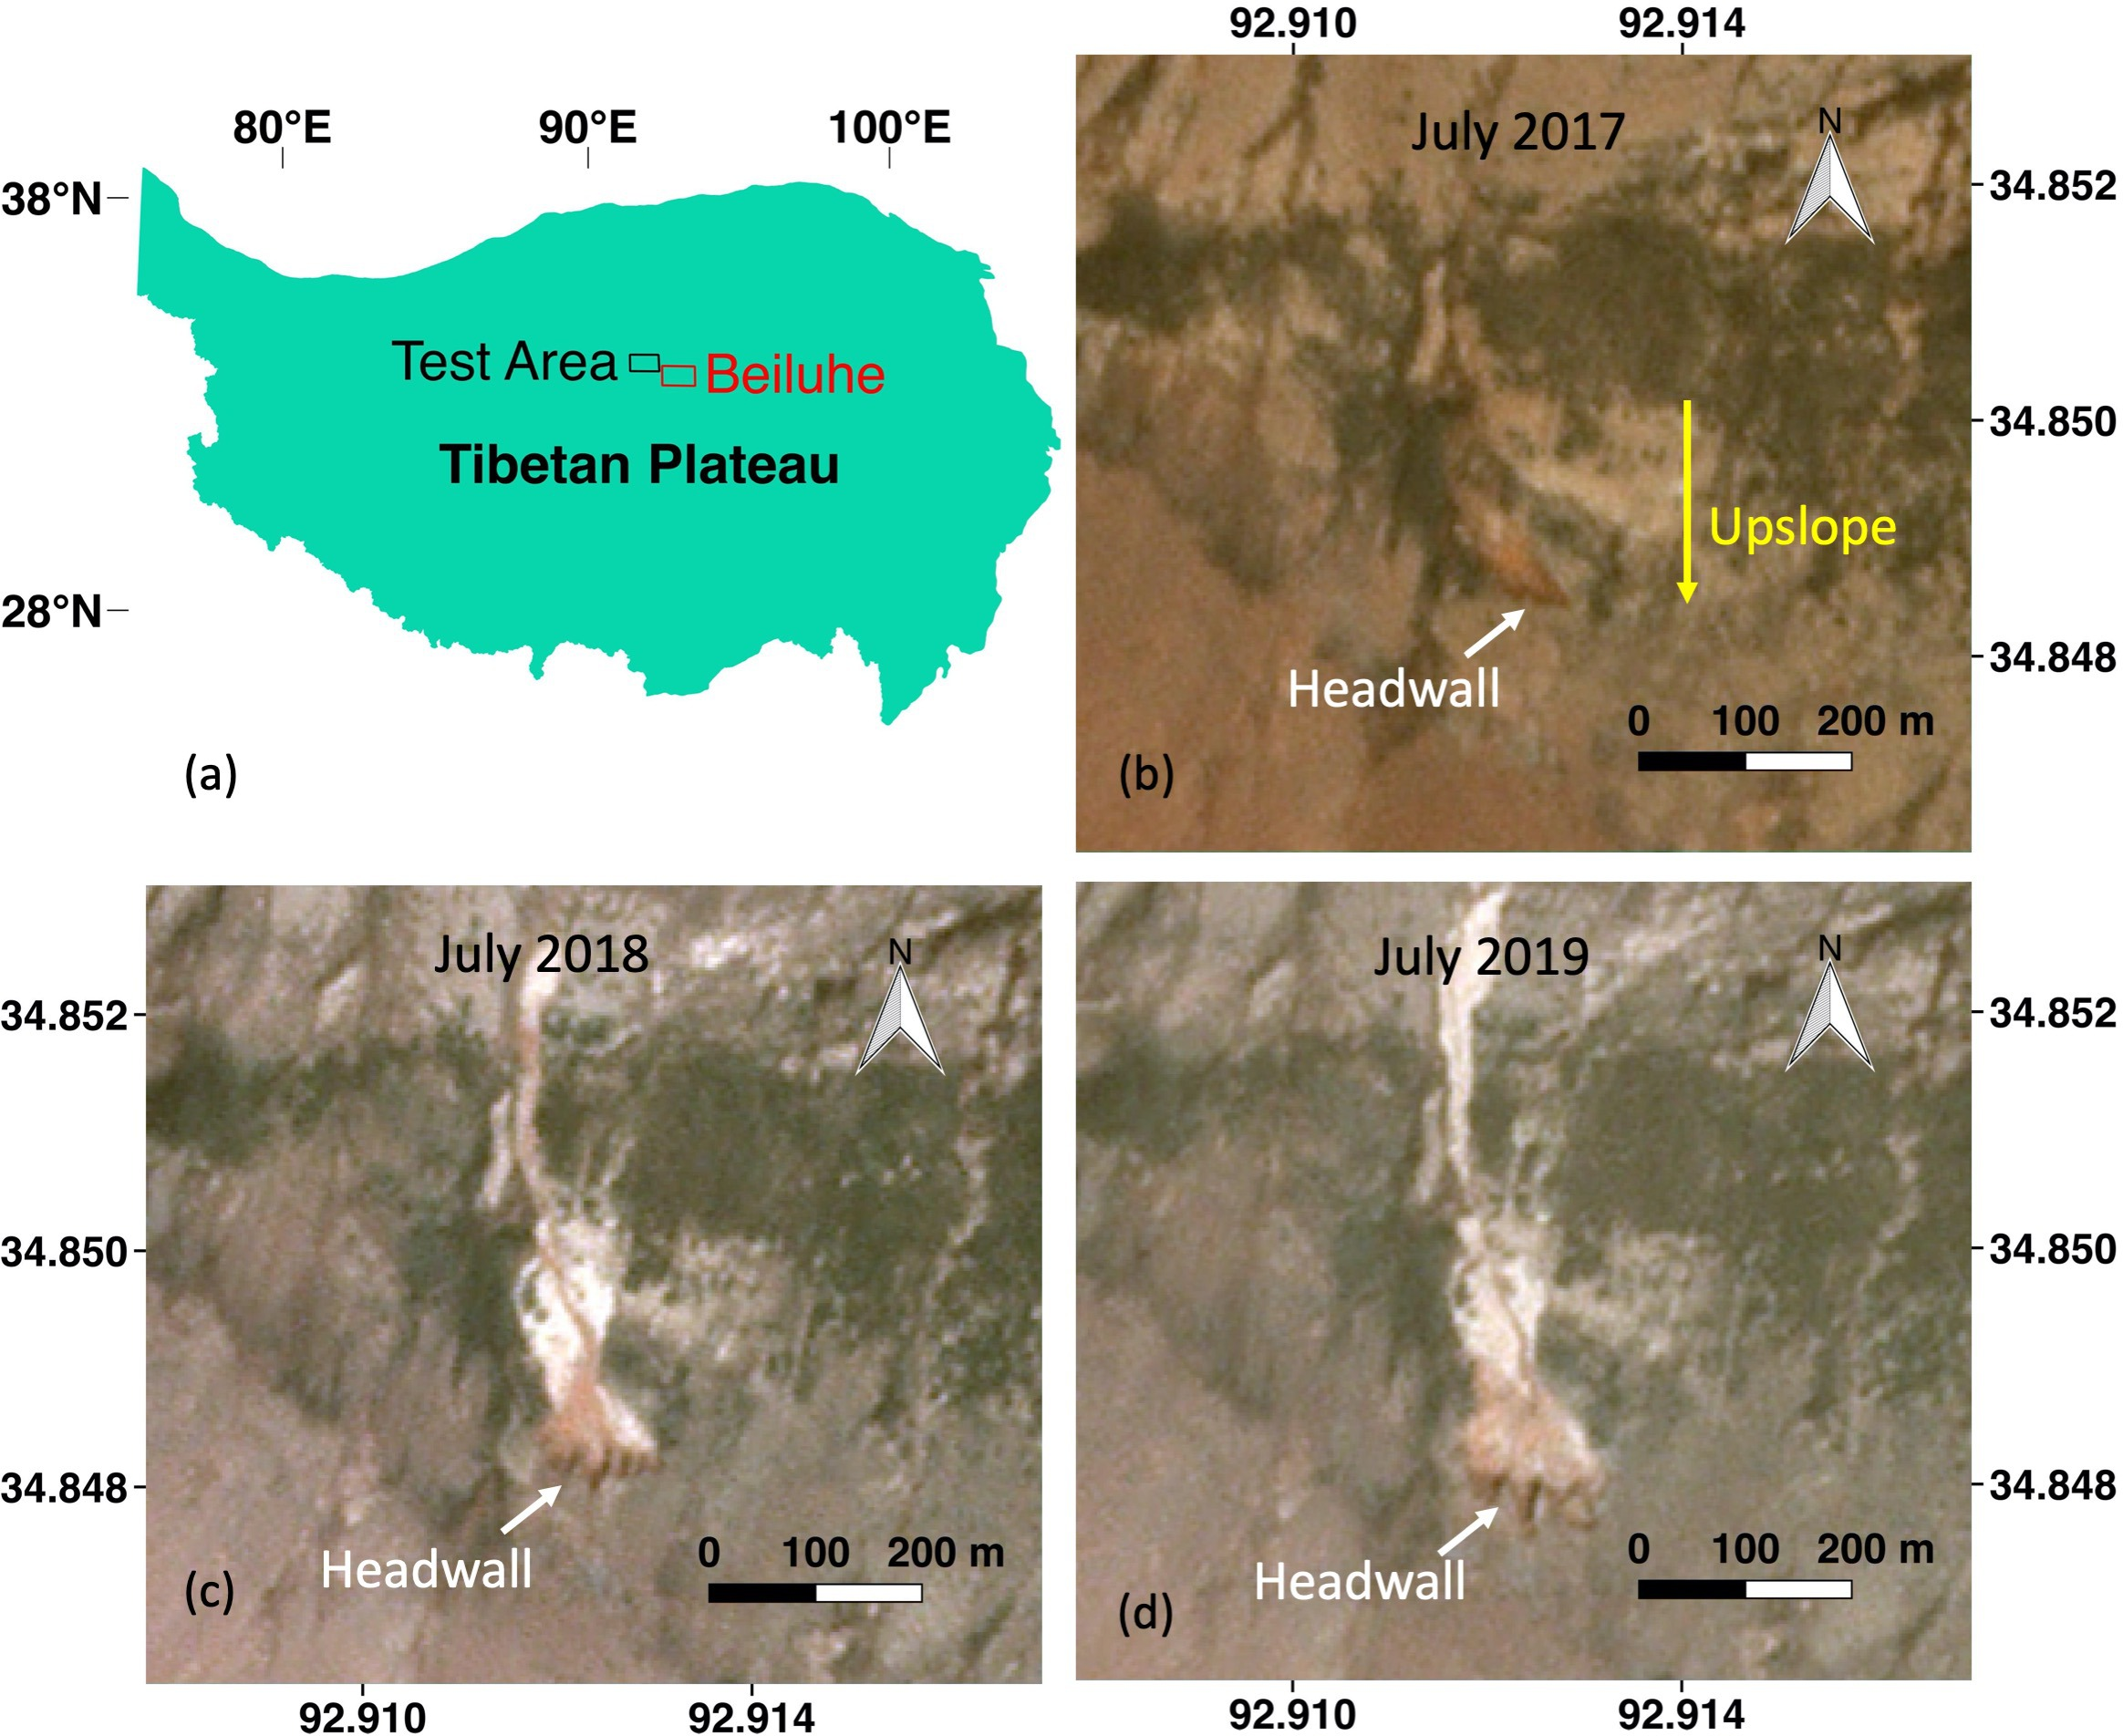
\includegraphics[width=14cm]{figs/rts_multi_images_study_area_v2_trim.jpg}
	\caption{The study area and development of a retrogressive thaw slump (RTS). The red 
	%and black 
	rectangle in (a) shows the extent of our study area
	% and test area 
	on the Tibetan Plateau. (b) to (d) are Planet images taken in 2017, 2018, and 2019 of an RTS whose central location is 92.912$^\circ$ E, 34.848$^\circ$ N. The white arrows point to the headwall which retreated upslope (as shown in the video in the Supplementary Materials).} % In (b), the yellow arrow indicates the upslope direction.
	\label{fig_multi_rts_image_studyarea}
\end{figure}


%Data
The core data are images taken in July 2017, 2018, and 2019 by the PlanetScope satellites.
%address why only choose the images starting from 2017? 
We use images after 2017 because images from the PlanetScope CubeSat are only available after that time in our study area.  
In July, vegetation reaches its maximum coverage, and active RTSs are in a rapid stage of thawing processes. 
Therefore, identifying RTSs would be relatively easy during this period.
These images have four bands (blue, green, red, and near-infrared) with a spatial resolution of 3 m, and each of them covers an approximate area of 10 km by 30 km.
Table \ref{table_image_list} lists the numbers and acquisition dates of these images. 
Because of the variation of cloud cover and image coverage, the image counts in different years are different.
They were downloaded from the Planet website (\url{www.planet.com}) or through a python package (\url{pypi.org/project/planet}) for Planet's public API under its Education and Research Program \citep{team2018planet}. 
The product level of images is ``Analytic\_SR'', which means that they had been orthorectified with a positional accuracy of 10 m, the pixel values represent surface reflectance by using a bit depth of 16 bits. 

%The RTS boundaries are derived from manual delineation on Planet images using the same method proposed by \cite{huang2020using}, parts of which will be used for training our automatic method. 
%We consider all the RTS boundaries as ground truths in the validation step, and 70\% of them are cross-checked in the field in 2014 and 2018. %on other satellite images? 
%The steps of downloading as well as pre-processing of Planet images and collecting ground truths are presented by \cite{huang2020using}.


\begin{table}[ht]
\footnotesize
\caption{Number and acquisition dates of images from the Planetscope satellites.}
\label{table_image_list}
\centering
%% \tablesize{} %% You can specify the fontsize here, e.g. \tablesize{\footnotesize}. If commented out \small will be used.
%\begin{tabular}{cc m{2.2cm}  m{2.2cm}  m{2.2cm} ccc}
%\begin{tabular}{c  c  m{2.5cm}   c m{3.0cm} }	% for 5 columns
\begin{tabular}{c  c    c  }	% for 5 columns
\toprule
% \multirow{2}{*}{ \textbf{Year/Month}}  & \multicolumn{2}{c}{ \textbf{Beiluhe}} &  \multicolumn{2}{c}{ \textbf{Test Area}}\\
% & Count & Acquisition dates & Count & Acquisition dates \\
%\midrule
% 2017 July & 71 & 17, 19, and 20 & 36 & 19 and 20 \\
% 2018 July & 52 & 20, 24, and 25 & 33 & 15 and 16 \\
% 2019 July & 46 & 25, 27, and 30 & 53 &  8, 24, 25, 27, and 30\\

Year & Acquisition dates & Number  \\
\midrule
2017  & July 17, 19, and 20  & 71 \\
2018  & July 20, 24, and 25  & 52 \\
2019   & July 25, 27, and 30 & 46 \\

\bottomrule
\end{tabular}

%\raggedright \#: the continuous experiment number
\end{table}


\section{Methods}
\label{sec_meth}

% the flowchart. 
\begin{figure}
	\centering
	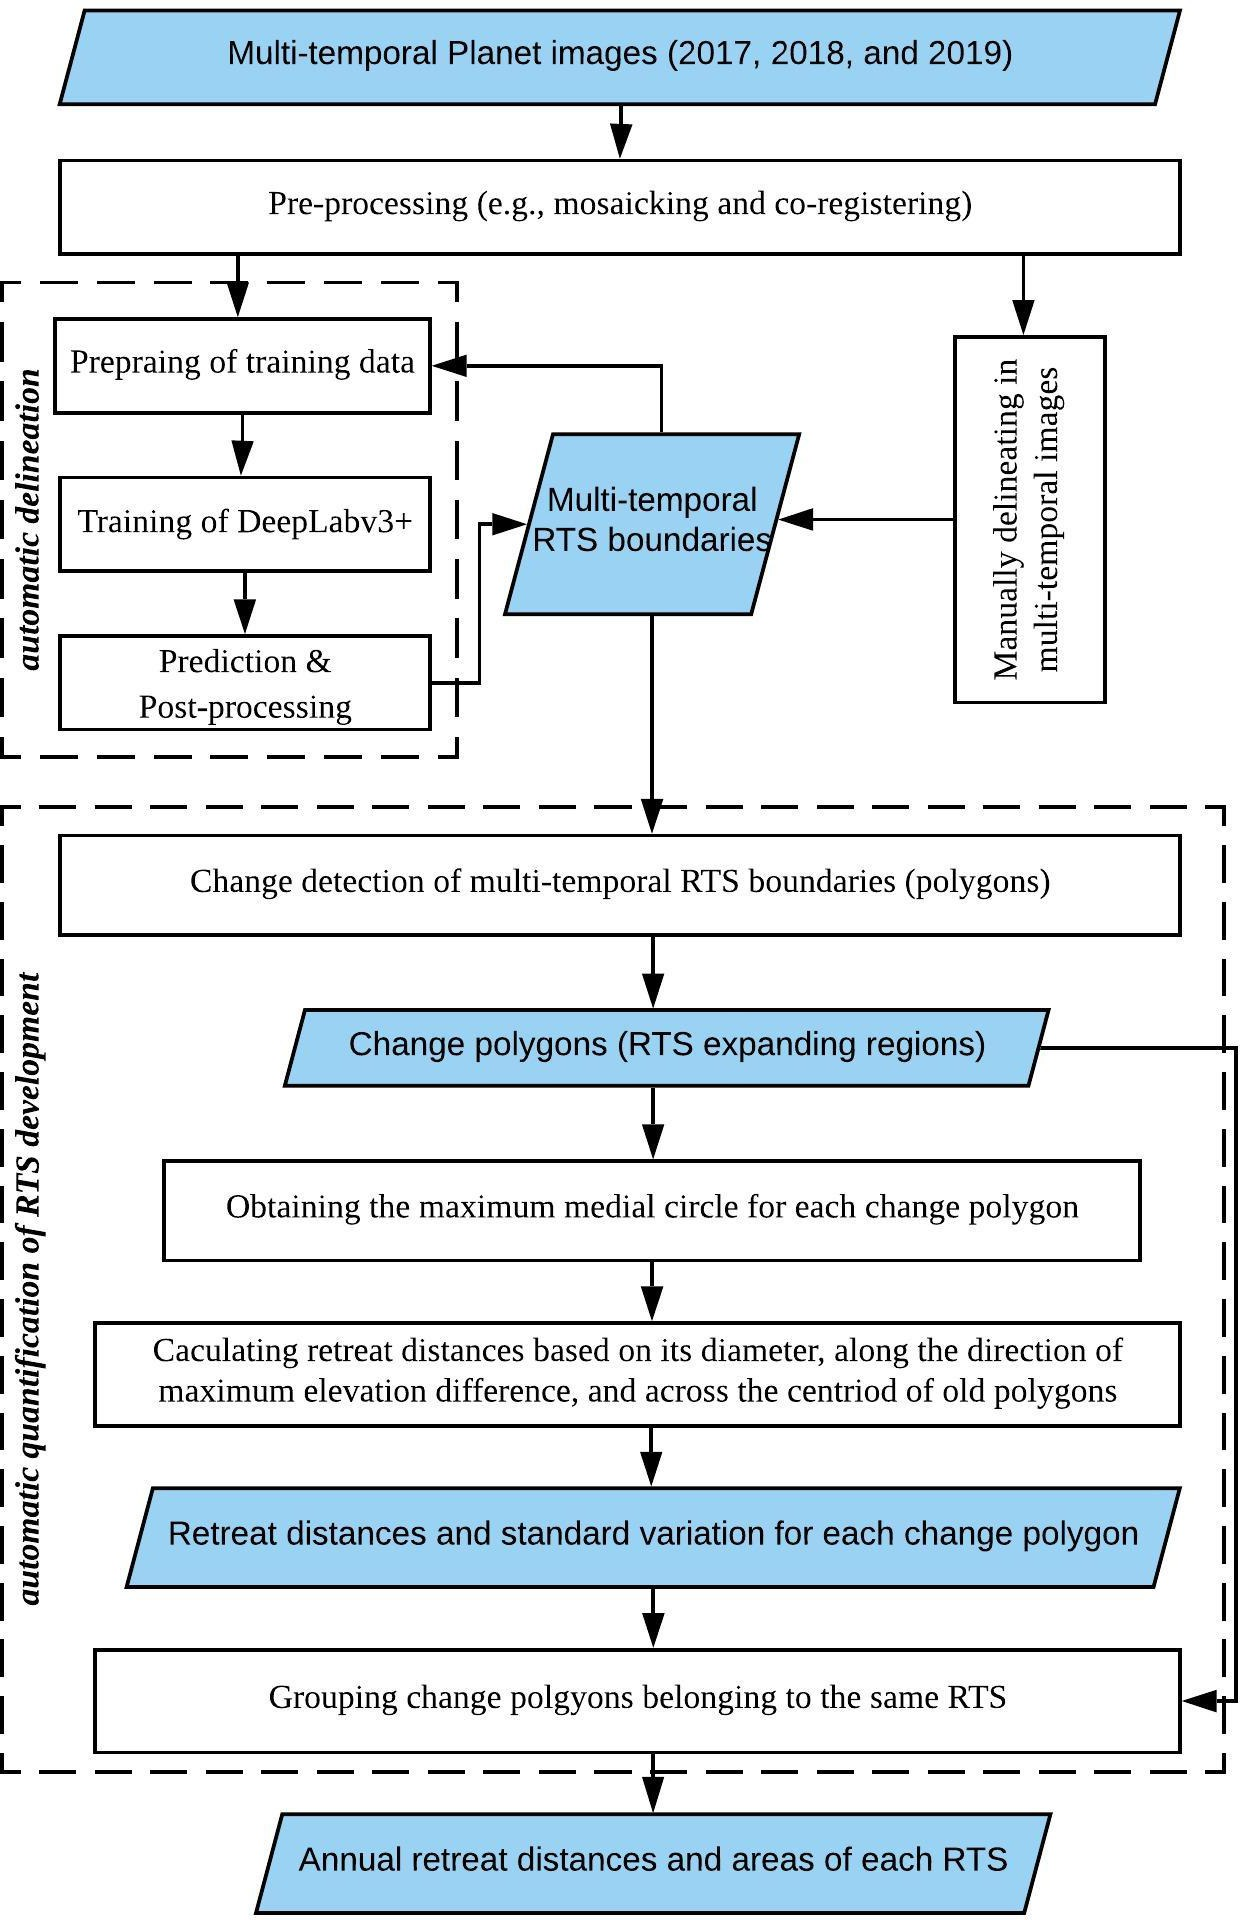
\includegraphics[width=9cm]{figs/polygon_based_change_detection_flowchart.jpg}
	\caption{Flowchart of automatic quantification of RTS development on multi-temporal images. The automated process includes three sections: (1) pre-processing of multi-temporal Planet images, (2) automatic delineation, and (3) automatic quantification of RTS development.}
	\label{fig_flowchart}
\end{figure}

 As shown in Fig. \ref{fig_flowchart}, the major procedures of the automatic method for quantifying RTS evolution include pre-processing of Planet images, automatic delineation of RTS, and automatic quantification of their development. 
Manual delineation of RTSs is necessary when data are not available to train DeepLabv3+, a supervised learning algorithm, because multi-temporal RTS boundaries are one of the key components of training data.
The automatic quantification accepts multi-temporal RTS boundaries, either derived from automatic or manual delineation, and would produce annual retreat distances and areas of each RTS. 


\subsection{Pre-processing of multi-temporal images}
\label{sec_preprocessing}

We pre-processed Planet CubeSat images to fulfil the requirements of DeepLabv3+ as well as manual delineation and to reduce the offset between multi-temporal images. 
For the images of each year, we pre-processed them by band extracting, stretching, sharpening, and mosaicking then obtained a mosaic image covering the study area. 
%Co-registration
To increase the relative positional accuracy (reduce the offset between multi-temporal images) among multi-temporal images, we apply co-registration to the three mosaic images from 2017 to 2019. 
Firstly, we chose the well pre-processed image \citep{huang2020using} as the reference image. 
Secondly, we used the scale-invariant feature transform algorithm \citep{lowe2004distinctive} with a GPU implement (\url{https://github.com/pitzer/SiftGPU}) to automatically find tie-points between %other
 mosaic images and the reference image \citep{huang2016a}. 
Lastly, we warped these images by using the Geospatial Data Abstraction Library (GDAL) with a first-order polynomial model.
% add co-registration accuracy in the supplementary files, also mentioned original 10 m accuracy 
As shown in Table S1 in the Supplementary Materials, the relative positional accuracies between images after co-registration are around 0.2 pixels, that is, 0.6 m. 


% test histogram normalization in pre-processing steps (as noted, the histogram normalization did not improve the quality of Planet images, so we may just skip further steps)

\subsection{Manually delineating RTSs on multi-temporal images}
\label{sec_manu_delineating}

We manually delineated RTS boundaries on multi-temporal images throughout the study area in QGIS (version 2.18.14, \url{qgis.org}). 
Based on the square grids and mapping results presented by \cite{huang2020using}, we delineated RTS boundaries on Planet images taken in all the three years as accurately as possible. 
The error (uncertainty) of manual delineation on Planet images is around one pixel, that is, 3 m. 
After the delineation, we obtain 338, 342, and 344 RTS boundaries on images from 2017 to 2019. 
The RTS numbers in this paper are larger than the one presented in \cite{huang2020using} by around 80 because multi-temporal images with better vegetation coverage enable us to identify many small and subtle RTSs. 
Two RTSs initiated in 2019 and captured by the 2019 image, but we removed them in the step of change detection (section \ref{sec_polygon_change_det}) because it needs at least two boundaries at the same location. 
Parts of these RTS boundaries will be used for training our automatic delineation method, and all of them would be considered as ground truths for validation. 
The locations of 55\% RTSs were cross-checked in the field in 2014 and 2018 and most of them  appear on other satellite images including WorldView-1, SPOT-5, and Gaofen-1 \citep{luo2019recent}. 
%
% parts of which will be used for training our automatic method. 
%We consider all the RTS boundaries as ground truths in the validation step, and 70\% of them are cross-checked in the field in 2014 and 2018. %on other satellite images? 
%The field work only validate the occurrence of RTS, not their boundaries. 



\subsection{Automatic delineation of RTSs on multi-temporal images}
\label{sec_auto_delineating}

To automatically obtain RTSs boundaries in different years, we applied DeepLabv3+ to multi-temporal Planet images. 
DeepLabv3+, one of the best algorithms for assigning each pixel a class label, is built on deep convolutional neural networks \citep{chen2018encoder-decoder} and outperforms (first place) many other algorithms in the PASCAL VOC image segmentation tasks \citep{everingham2015The}.
Moreover, \cite{huang2020using} have proved that a well-trained DeepLabv3+ model can delineate RTSs and obtain their boundaries that are very close to manual delineation.
The steps of automatic delineation include preparing training data, training a DeepLabv3+ model, delineating RTS boundaries, and validation as detailed below. 
%We used a deep-learning-based algorithm \citep{huang2020using} to automatically delineate RTSs on multi-temporal images.
%Compared with the method in \cite{huang2020using},  the innovation of this work includes (1) training without using negative training polygons and (2) improving RTS mapping results by utilizing RTS dynamic information in multi-temporal images. 
%The details will be presented as the following.

% not include negative training polygons, has bad results, but can be removed by the multi-temporal information. 

\subsubsection{Preparing training data}
\label{sec_prepare_training}

%\subsubsection{Training a single model} 
%\label{sec_training_model}

% Preparing training data

We derived training data that can be input into DeepLabv3+ directly from training polygons and selected Planet images.
The training polygons consist of parts of the ground truths (i.e., positive training polygons) and polygons covering non-RTS regions (termed as negative training polygons) in different years.
These negative training polygons are necessary for distinguishing land covers (e.g., bare land) that are similar to RTSs but need ground information or some initial tests to generate them. 
Based on our initial test, we drew 78 negative training polygons and duplicated them to different years if necessary. 
We chose all the ground truths as well as negative training polygons for training. 
To assess the capability and generalization of DeepLabv3+ when applied to multi-temporal Planet images, we conducted experiments using (1) ground truths of 2017 and 2018 as well as 78 negative training polygons for training and (2) all ground truths but without negative training polygons.
%We considered all the ground truths as positive training polygons but did not include any negative training polygons. 
%However, generating negative training polygons will be impractical for mapping RTSs in a large area. 
%need to check this sentence, may not right. have checked, it is right, it happened in Beiluhe 
We conducted experiments without negative training polygons because (1) it takes efforts to generate them and (2) they may cover areas with emerging RTSs or expanding parts of RTSs captured by images taken in a later time. 
%Therefore, we excluded negative training polygons for the training of DeepLabv3+ when applying to multi-temporal images.
Without negative training polygons, the mapping results may contain many false positives, but we can utilize the RTS dynamic information in multi-temporal images to remove them (see section \ref{sec_improving_using_rts_dynamic}).


For the training polygons and Planet images in each year, we extracted sub-images with a buffer area of 300 m. 
Then we subdivided all sub-images into patches by setting a patch size as 480 pixels with an overlap of 160 pixels. 
Details of the extracting and subdividing operation are presented by \cite{huang2018automatic}.
To improve the volume of training data and generalization of the trained model, we applied data augmentation (flipping, blurring, cropping, and scaling) to the patches. 
Lastly, we considered all the patches from different years as a single training dataset. 


%\subsubsection{Training a model and delineating RTSs on multi-temporal images}
%\label{sec_train_prediction}

%\subsubsection{Training a model, delineating, and post-processing}
\subsubsection{Training, delineating, and post-processing}
\label{sec_train_deli_post_pro}

% training
We trained a DeepLabv3+ model (i.e., network parameters) by using the training data derived in section \ref{sec_prepare_training}. 
Instead of training different models for different years, we only trained a single model because DeepLabv3+ has a high capability to represent RTS features on multi-temporal images. 
Moreover, the strategy of a generic model is more convenient and efficient than the one of the multiple models when expanding in the time domain. % can save a lot of computing resources, especially
The network architecture and pre-trained model we used were Xception65 \citep{chollet2017xception} and based on the ImageNet datasets \citep{russakovsky2015imagenet}, respectively. 
The hyper-parameters such as the learning rate (0.007), batch size (8), and iteration number (30000) were the same as the ones used by \cite{huang2020using}.

%In this study, instead of training different models for different years, we only trained a single model because DeepLabv3+ has a high capability to represent RTS features in multi-temporal images, more importantly, a generic model can save a lot of computing resources, especially when expanding the time domain.
%We used the same hyper-parameters presented in \cite{huang2020using} when training this model. 
%To evaluate the robustness of the model, we utilized k-fold cross-validation (k=3, 5, and 10)  as commonly used in machine learning. 

 %How about the test Area? use which trained model?  not include the test area. 
%k-fold cross-validation. 

% prediction (delineation)
We used the trained model to delineate (predict) RTSs on the 2017, 2018, and 2019 mosaic images. 
The steps of delineating RTSs on each mosaic image include
(1) dividing it into numerous small patches (each with a size of 480 $\times$ 480 pixels and an overlap of 160 pixels with its adjacent ones),
(2) predicting RTS or non-RTS pixels and obtaining a binary patch,
(3) mosaicked the binary patches using GDAL and obtained a binary mosaic, and % post-processing
(4) polygonizing the binary mosaic.  % post-processing
%The size and overlap of each patch for prediction is the same as the one for preparing training data (section \ref{sec_prepare_training}). 
To improve computational efficiency, we adopted a parallel strategy, that is, assigning different mosaic images to different GPUs for running the delineation process simultaneously. 
After the polygonizing, we obtained polygons (termed as mapped polygons afterward) which represent locations and boundaries of RTSs predict by the trained model. 
% % this is a step of post-processing
Lastly, considering the image resolution, we removed mapped polygons with an area smaller than 0.09 ha (100 pixels). % 0.3 ha.

\subsubsection{Removing erroneously mapped polygons using the RTS dynamic feature}
%\paragraph{Improving RTS mapping results using the RTS dynamic feature}
\label{sec_improving_using_rts_dynamic}


Many mapped polygons were erroneously identified as RTS polygons can be removed by utilizing the RTS dynamic feature. 
As shown in Fig. \ref{fig_rts_expanding}, an active RTS can expand toward upslope annually, even for a non-active RTS, its extent cannot shrink. 
Therefore, we can use this dynamic feature to remove non-RTS mapped polygons. 
Firstly, we obtained a union (Fig. \ref{fig_rts_expanding}) of mapped polygons at the same location.
The steps of obtaining the union include (1) choosing a mapped polygon as an initial union, (2) scanning through all mapped polygons until finding a mapped polygon that has not been merged to other unions and overlaps it, (3) merging the found polygon into it and updating the union, and (4) repeating steps (2) and (3) until no polygons can be merged into the union. 
Secondly, we calculated the intersection over union (IOU) for mapped polygons in each year (termed as ``time-IOU") as follows, 
\begin{equation}
IOU(A,B)_{t}=area(A \cap B)/area(A \cup B)
\label{equ_time_iou}
\end{equation}
where \emph{A} is a mapped polygon in the specific year, \emph{B} is the union, and \emph{t} is the time. 
Due to the expanding dynamics of RTSs, the time-IOU of an active RTS should monotonically increase over time. 
If an RTS is already stabilized, its time-IOU will remain the same over time. 
Considering the delineation error (e.g., the RTS boundaries in different years at non-headwall parts do not exactly overlap each other as shown in Figs. \ref{fig_rts_expanding} and \ref{fig_rts_change_det}), a relaxed threshold of $-0.1$ was set to determine if the time-IOU of an RTS is monotonically increasing, that is, if all the differences ($IOU_{next\_year}-IOU_{year}$) are greater than $-0.1$.% we consider the time-IOU is monotonically increasing. 
Thirdly, because most of the RTSs in the Beiluhe region initiated in or before 2016,
we can assume that at a specific location where an RTS emerges, it presents at least two mapped polygons from 2017 to 2019 with time consecutiveness, referred to as the ``two-polygon assumption''. 
Lastly, we removed mapped polygons in a location that does not satisfy the two-polygon assumption or the time-IOU is not monotonically increasing.
 
%[ht]
\begin{figure} 
	\centering
	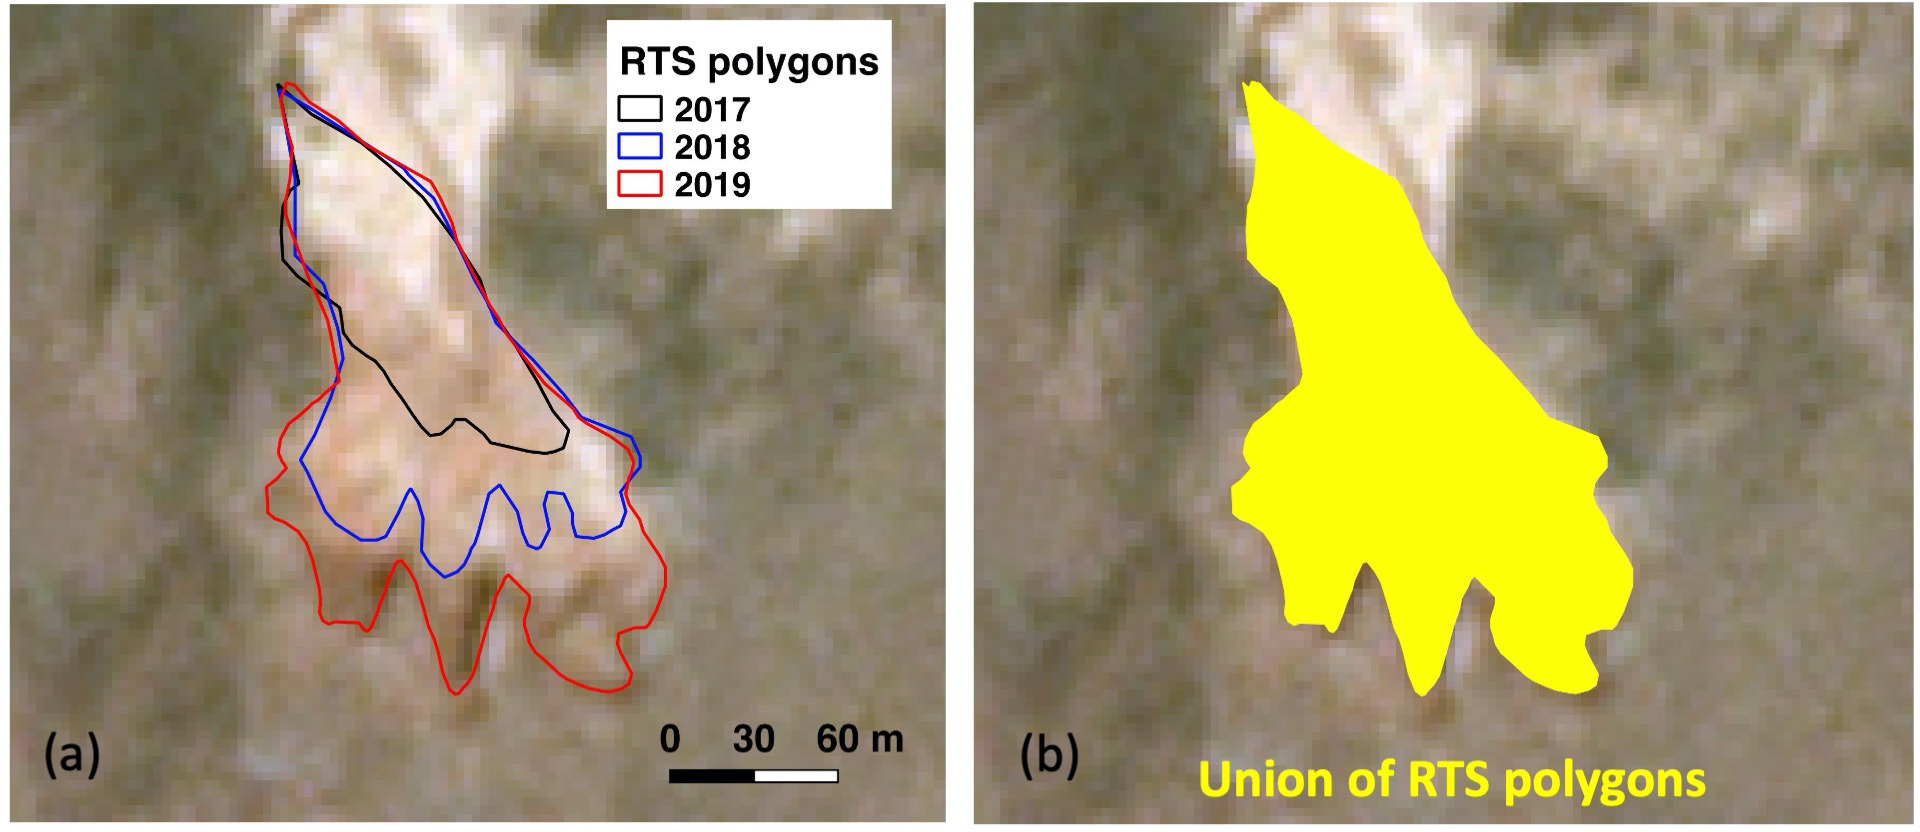
\includegraphics[width=14cm]{figs/rts_expanding_example_trim.jpg}
	\caption{RTS polygons (a) representing their boundaries from 2017 to 2019 and the union (b) of these polygons. The background is 2019 Planet images, and the RTS is the same as the one shown in Fig. \ref{fig_multi_rts_image_studyarea}}
	\label{fig_rts_expanding}
\end{figure}


\subsubsection{Validating mapped polygons}
\label{sec_validate_mapped_polygons}

To validate the mapped polygons, we calculate their F1 scores in each year separately. 
For each year, we calculate IOU values between the mapped polygons and the corresponding ground truths. 
We set a threshold of 0.5 to decide a mapped polygon is a false positive (FP) or true positive (TP).
After obtaining the counts of true positives, false positives, and false negatives (FN), we can calculate the precision and recall, then calculate the F1 score using the following equation. 
\begin{equation}
F1=2 \times Precision \times Recall / (Precision + Recall)
\label{equ_f1score}
\end{equation}
More details of the F1 score and its implication can be found in \cite{huang2020using}.
We repeated the calculation of F1 scores for different years and obtained the corresponding values. 
% did I calculate the average of three AP? It seems no.
To assess the performance of the delineating method in this paper, we calculated the average precision (AP) values for mapping results in different years. %, then averaged them. 
AP values are based on precision-recall curves which is an effective metric for evaluating the algorithm performance \citep{huang2020using}.
%A higher average of AP values indicates the better performance of the method. 
A higher AP value indicates the better performance of the method. 

%\subsection{Detecting temporal changes of RTS boundaries}
%\label{sec_detect_rts_changes}
\subsection{Automatic quantification of RTS development}
\label{sec_auto_rts_develop}

To automatically quantify RTS development with the input of RTS boundaries, we proposed a method to detect changes of RTS boundaries and calculate their annual retreat distances.
The RTS boundaries are in vector format and can be derived from manual or automatic delineation. 
The main steps include polygon-based change detection, removing false changes, and calculating retreat distance as detailed below. 

\subsubsection{Change detection of RTS boundaries}
\label{sec_polygon_change_det}

%a figure showing a multiPolygon and its narrow parts. 
%[ht]
\begin{figure} 
	\centering
	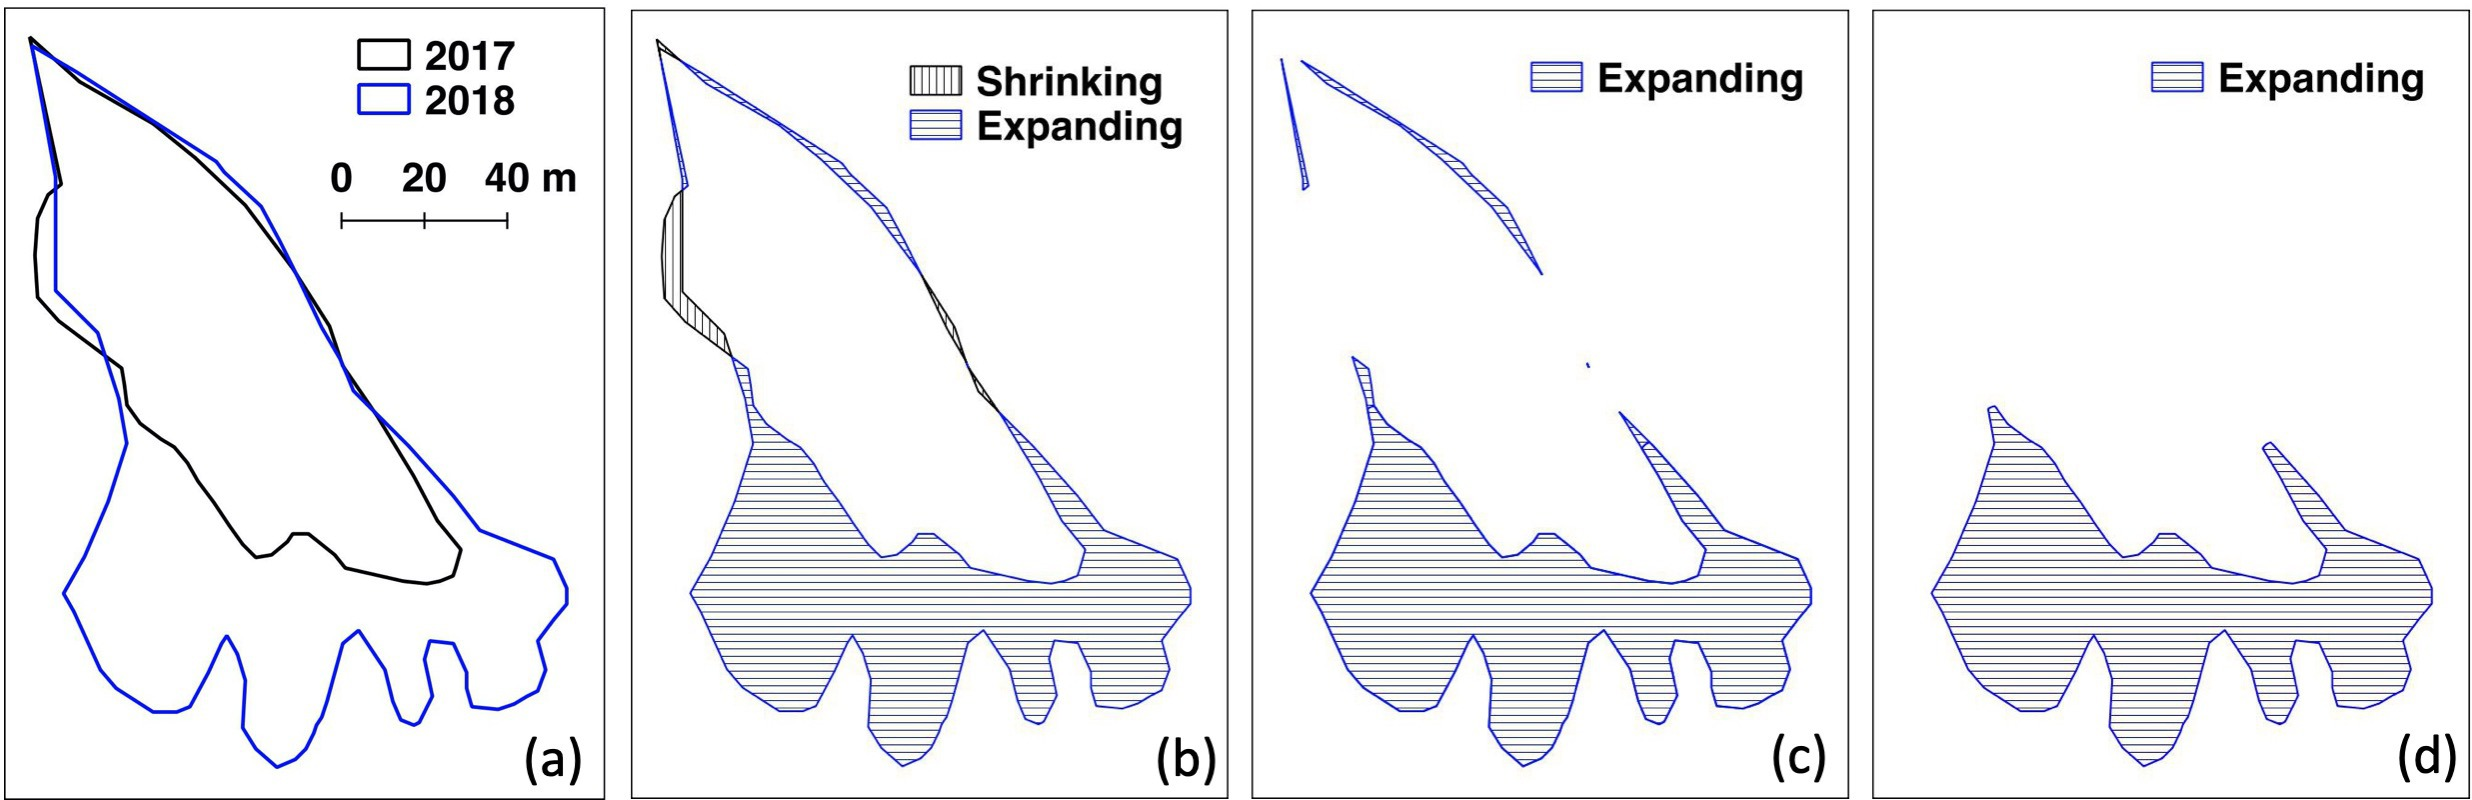
\includegraphics[width=14cm]{figs/rts_polygon_change_det_trim.jpg}
	\caption{An example of the polygon-based change detection. (a) shows the boundaries of an RTS (Fig. \ref{fig_rts_expanding}a) in 2017 and 2018. $P_{2018}-P_{2017}$ results in an expanding multiPolygon (b) and the corresponding non-narrow parts (c). $P_{2017}-P_{2018}$ results in a shrinking multiPolygon (d).}
	\label{fig_rts_change_det}
\end{figure}

To obtain the annual RTS changes, we conducted change detection for RTS boundaries between one year and its previous year.%, that is, comparing 2018 with 2017 and 2019 with 2018. 
 As indicated in Equation \ref{equ_polygon_diff}, for a specific location containing RTS polygons in different years, a polygon in this year minus the one in the previous year should result in expanding regions. 
We used the ``difference'' function in Shapely (\url{https://pypi.org/project/Shapely}) to implement the subtraction in Equation \ref{equ_polygon_diff}. 
The expanding regions were represented as geometries with type of ``Polygon'' or ``multiPolygon'' in Shapely.
\begin{equation}
E_{t}= P_{t} - P_{t-1}
\label{equ_polygon_diff}
\end{equation}
% \emph{t} represents year: have said t in the equation equ_time_iou
where \emph{P} is an RTS boundary, \emph{E} is the expanding regions, and \emph{t} is the time. 
From the perspective of change detection, $P_{t}$ is a new polygon and $P_{t-1}$ is the corresponding old polygon at the same location. 
While $P_{t} - P_{t+1}$ can result in shrinking regions, which is caused by delineation errors. 
Fig. \ref{fig_rts_change_det} shows an example of the subtraction operation between the RTS boundaries in 2018 and 2017. 
%removing the narrow parts. 
Considering delineation errors and the resolution (3 m) of Planet images, we removed the narrow parts of expanding regions using buffer operation as follows, 
\begin{equation}
E_{non\text{-}narrow}= E.\text{buffer}(-r).\text{buffer}(r*f) \cap E
\label{equ_polygon_buffer}
\end{equation}
%\emph{E} is a polygon or multiPolygon,
where \emph{r} is the value of buffer operation,  \emph{f} is a factor between 1 to 2 for avoiding uncertainties of buffer operation. 
% check or update the r and f value in the codes, I did
In this study, we set \emph{r} as 3 and \emph{f} as 1.6 after initial experiments and used the ``buffer'' function in Shapely.
To make it practical for calculating polygon attributes (e.g., area and perimeter) and removing false changes (section \ref{sec_removing_false_change}), we converted all the expanding regions to many separate polygons (termed as change polygons), that is, converting geometries with multiPolygon to polygons.



%a multi-polygon to polygons and calculate the attributes: area, circularity, 
%zeroIntersection, two or more intersections, holes, relative elevation, retreat distance. 

\subsubsection{Removing false change polygons}
\label{sec_removing_false_change}

%in this section, some threshold for removing operation need to confirm in codes or more experiments. 
%Polygon change detection. \\\\
This step utilized pre-set criteria to remove change polygons that are possibly incorrect. 
%  check using ha or m^2 
Firstly, we removed a change polygon if its area is smaller than 36 $m^2$ or greater than 50000 $m^2$. 
%minimum_change_area = 36
%maximum_change_area = 50000
The reasons for setting these two thresholds are that (1) we assumed that minimum changes on Planet images are $2\times2$ pixels, that is, 36 $m^2$ and (2) as reported by \cite{huang2020using}, 90\% RTSs in Beiluhe are smaller than 50000 $m^2$. 
%b_remove_polygons_with_holes = Yes
% bad mapping results, actually, but can not remove a few because previous steps have remove mapped polygons based on multi-temporal images. 
%TODO: need to discuss this in the discussion session.
%b_remove_zero_intersection = Yes
%b_remove_two_or_more_intersection = Yes
Secondly, a change polygon derived from erroneously mapped polygons was removed.
% these belong to previous section. No, we have revised it. 
We considered a mapped polygon as erroneous if it meets one of the following criteria: (1) containing holes, (2) not intersecting any mapped polygons in other years, or (3) intersecting two or more mapped polygons in other years.
Usually, these erroneous polygons are resulted from automatic mapping methods, and most of them would be removed after applying the RTS dynamic feature (section \ref{sec_improving_using_rts_dynamic}). 
%minimum_relative_elevation = 0
Thirdly, we removed change polygons if their elevation difference (Equation \ref{equ_elevation_diff}) is smaller than zero (i.e., not in the upslope zone). 
\begin{equation}
%Elevation_{diff}=Elevation_{ChangePolygon_{E_{t}} -  Elevation_{P_{t-1}}}
\Delta H = H_{C_{t}} -  H_{P_{t-1}}
\label{equ_elevation_diff}
\end{equation}
where $\Delta H$ is the elevation difference, $H$ is elevation, and $C_{t}$ is a change polygon at time $t$.
We used the 30 m digital elevation model (DEM) from the Shuttle Radar Topography Mission (SRTM) \citep{farr2007shuttle} for calculating the elevation difference. 
For a change polygon or RTS polygon, we chose the mean of elevation within it as its elevation. 
%minimum_retreat_distance = 6
Lastly, we set a threshold of 6 m for retreat distance (see section \ref{sec_cal_retreat_dis}) to remove change polygons with the consideration of Planet image resolution and delineation errors. 
%minimum_change_circularity = 0 (no effect )


\subsubsection{Calculating and validating retreat distance}
\label{sec_cal_retreat_dis}

% To calculate the retreat distance
We utilized medial circles, which are the inscribed circles contained in a change polygon and tangent to it in at least two points, to calculate the annual retreat distance of RTSs. 
A series of medial circles can represent the shape of any polygon, and their centers indicate the medial axis of the polygon \citep{zhu2014computing}, such as the circles and red lines in Fig. \ref{fig_retreat_dis}a. 
% as illustrated in Fig \ref{fig_retreat_dis},
Among these medial circles, the diameter of the maximum one is a good approximation for the retreat distance (Fig. \ref{fig_retreat_dis}b).
However, due to the irregular and complex  shapes of the change polygons, medial circles may underestimate the maximum retreat distance and cannot handle multiple retreat branches as well as ones with an extremely elongated shape. 
To assess the underestimation and provide supplement information of retreat distance, for each change polygon, we automatically 
drew two lines crossing the center of its maximum medial circle and calculate the distance based on these intersected line segments, as illustrated in Fig. \ref{fig_retreat_dis}c. 
The directions of the two lines are determined by (1) the direction of the maximum elevation difference and (2) from the centroid of the corresponding old polygon (i.e., $P_{t-1}$ in equation \ref{equ_polygon_diff}) to the center of the circle. 
The retreat distance based on the line segments tend to be overestimated but can provide additional information of automatic calculation such as confidence because their accuracies are highly sensitive to elevation accuracy and shape of the RTS boundary in the previous year (e.g., the old polygon in Fig. \ref{fig_retreat_dis}c). 
%The variation of these three distances can indicate the consistency of the three measurements mentioned above . %A small value of difference indicate high confidence, and vice versa. 
We calculated the standard deviation of the three distances for each RTS and used it as an indicator for confidence or consistency of automatic calculation. 
Usually, higher variations are the results of irregular shapes of change polygons.
For the case when an RTS contains several change polygons, we chose the maximum value as the RTS retreat distance.
%We calculate the variation based on the following equation: 
%\begin{equation}
%PlaceholderFOR=dis_{confidence}
%\label{equ_dis_confid}
%\end{equation}

%a figure showing a multiPolygon and its narrow parts. 
%[ht]
\begin{figure} 
	\centering
	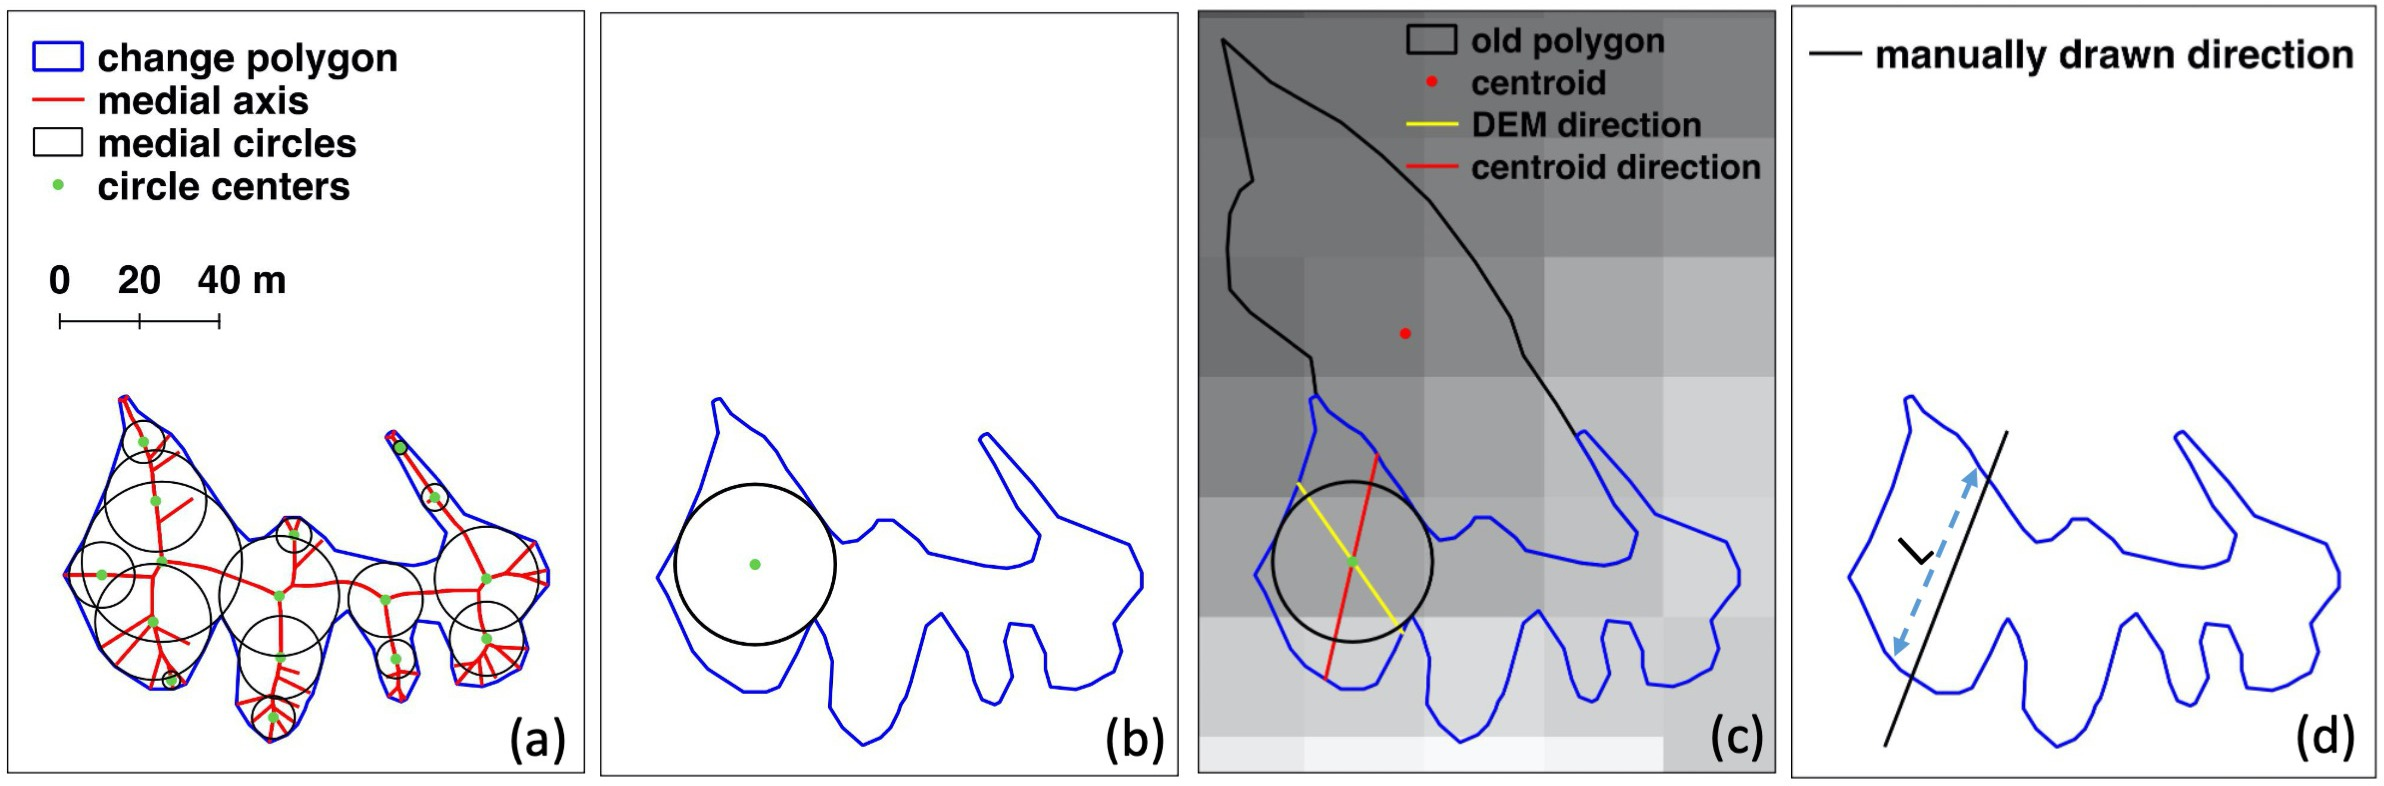
\includegraphics[width=14cm]{figs/retreat_distance_v2_trim.jpg}
	\caption{Calculating the retreat distance from a change polygon based on its medial axis and circles. (a) shows the medial axis (red lines) and some medial circles as well as circle centers (green dots). (b) shows the maximum medial circle whose diameter can be considered as the retreat distance. (c) shows other two approaches of choosing retreat direction: (1) along the direction of maximum elevation difference (indicated by the yellow line) and (2) from the centroid (the red dot) of the old polygon to the center of the maximum medial circle (indicated by the red line). The background in (c) is the SRTM elevation, and the brighter color indicates higher elevation (4695--4729 m). (d) shows a manually drawn line pointing the retreat direction, and based on which to derive the retreat distance $L$. }
	\label{fig_retreat_dis}
\end{figure}

% We used the algorithm medial circle \citep{zhu2014computing}.


%Step 1: got medial circles, sorted the circles by radius, resample the circles by  the data and find out what is the results. 

%We calculated the retreat distance for each change polygon based on its medial axis. 

% manually calculate the retreat distance by drawing a line indicating toward slope direction. 
% an RTS may have two or more branches, group RTS change polygons belongs to the same polygons. 
To validate the retreat distance, we manually drew a line indicating expanding direction of each RTS, and based on this line to its calculate retreat distance as ground truth ($L$), as shown in Fig. \ref{fig_retreat_dis}d. 
In cases where an RTS has more than one expanding branches, we chose the maximum one as its retreat distance. 



%\subsubsection{Validating RTS changes}
%\label{sec_validation_change}

\section{Results}
\label{sec_result}

%\subsection{The mapping performance when using multi-temporal images}
%\subsection{Mapping results in multi-temporal images}
%\label{sec_mapping_performance}

\subsection{Automatically delineating results on multi-temporal images}
\label{sec_result_auto_deliea}


\subsubsection{Mapped polygons and their accuracies} %in 2017, 2018, and 2019
\label{sec_mapped_polygons}

The mapped polygons accurately delineate most RTS boundaries on images taken in 2017, 2018, and 2019, with F1 scores of 0.820, 0.793, and 0.788, respectively.
Among the mapped polygons, around two-thirds of them are true positives (black, blue, and red polygons in Fig. \ref{fig_mapping_results}), and the rest are false positives (yellow polygons in Fig. \ref{fig_mapping_results}). 
Details of these numbers are presented in Table \ref{table_accuracy_f1} (rows of RTS-dynamic).
The distribution of mapped polygons for the entire Beiluhe region is shown in Fig. \ref{fig_mapping_results}a, and amplifications of three locations are shown in Fig. \ref{fig_mapping_results}b--d. 
Compared with the ground truths presented in Fig. S1 in the Supplementary Materials,  around 90 RTSs are missed in the mapped polygons such as the three within the yellow rectangle in Fig. \ref{fig_mapping_results}b.
As shown in Fig. \ref{fig_mapping_results}c and d, the true positives are close to the ground truths, that is, the automatically delineated ones are similar to the ones from manual delineation. 

%%%%%%%%%%%%%%%%%%%%%%%%%%%%%%%%%%%%%%%%%%%%% 
%%%% put the mapped polygons in Test Area to Supplementary Materials??? %%%%
%%%%  However,  the results for test area are not good (F1 score around 0.1), maybe it's ok to exclude the test area in this manuscript. The focus of this manuscript is the polygon-based detection, not mapping, the get the retreat distance automatically. Also, the performance of DeepLabv3+ has been proved in the previous RES paper.
%%%%%%%%%%%%%%%%%%%%%%%%%%%%%%%%%%%%%%%%%%%%%%



%%%%%%% Mapping results from exp7 %%%%%%%%%%%%%
\begin{figure} 
	\centering
	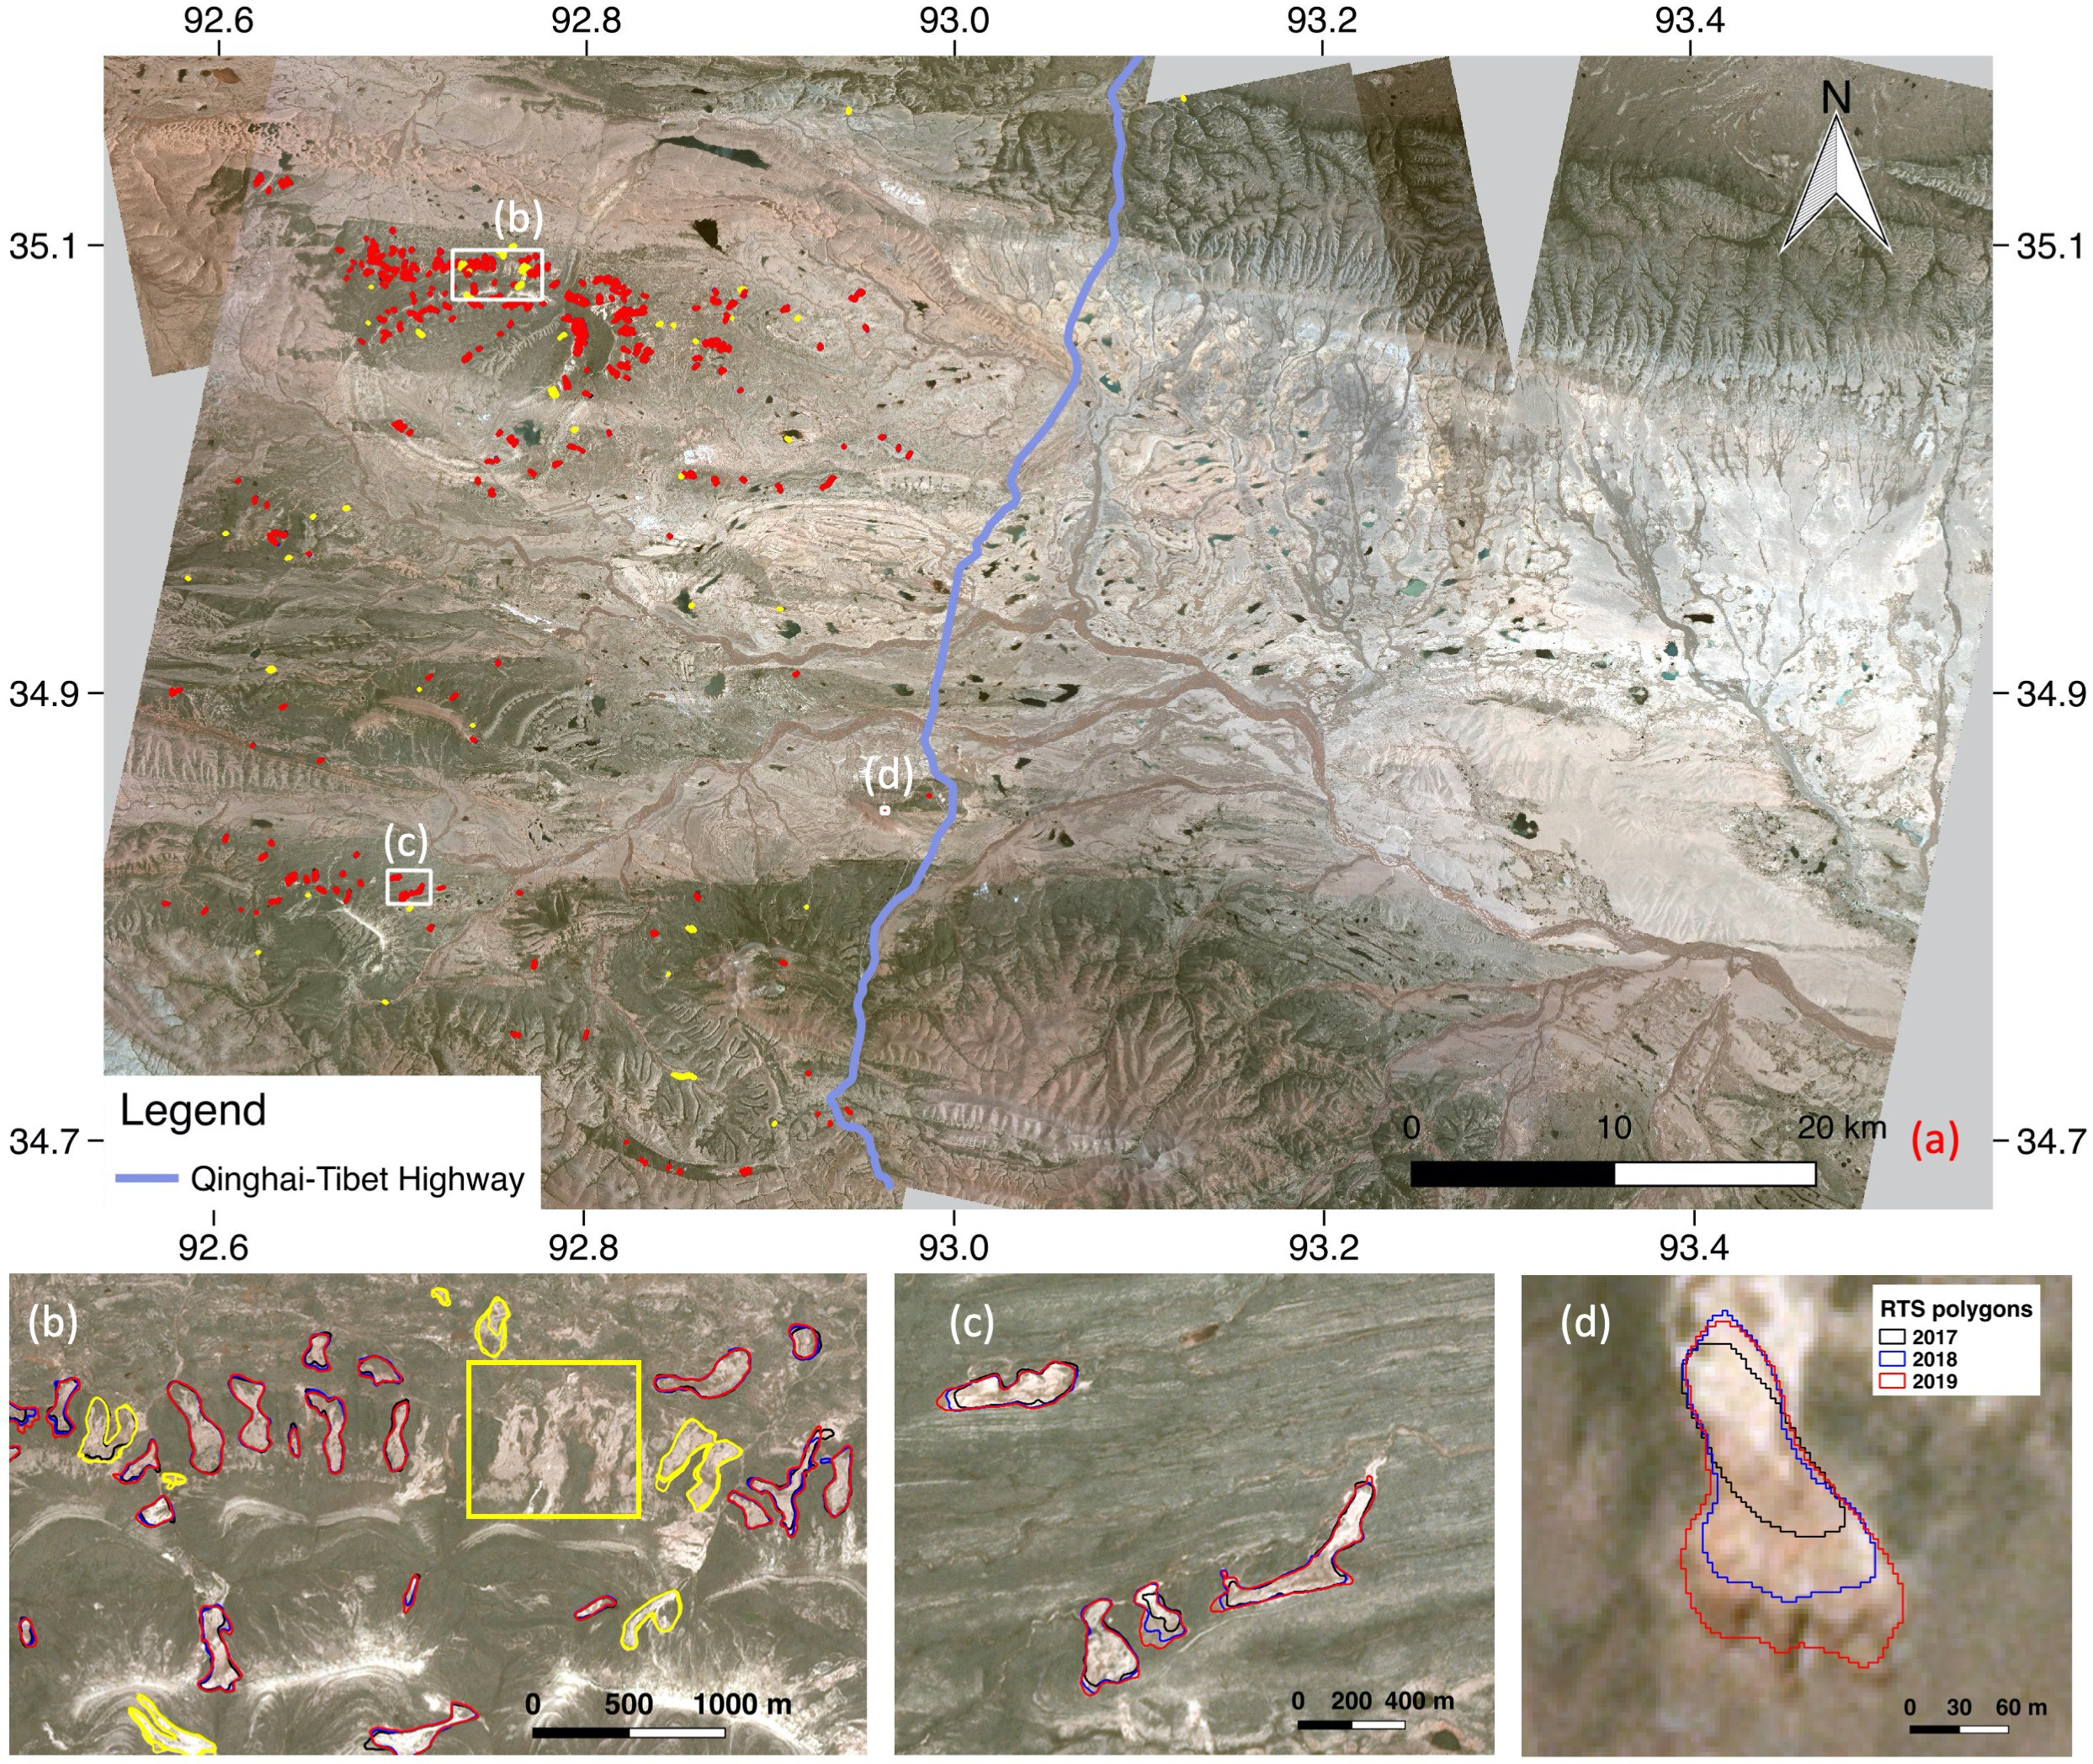
\includegraphics[width=14cm]{figs/multi_mapping_results_v2_trim.jpg}
	\caption{Mapped polygons in different years with applying RTS dynamic features. The black, blue, and red polygons are true positives delineated in the 2017, 2018, and 2019 images, respectively, while the yellow ones are false  positives. The background is the mosaic of 2019 Planet images. (a) shows the results in the entire Beiluhe region, and (b)--(d) are amplifications of three regions marked by rectangles in (a). The yellow rectangle in (b) marks three missed RTSs by the method. (d) shows the same RTS in Fig. \ref{fig_multi_rts_image_studyarea} and \ref{fig_rts_expanding} but with boundaries from automatic delineation.}
	\label{fig_mapping_results}
\end{figure}

%%%%%%%% Mapping results from exp7 %%%%%%%%%%%%%
%\begin{table}[ht]
%\footnotesize
%  \centering
%  \caption{Accuracy of mapped polygons in 2017, 2018, and 2019, respectively, with and without considering RTS dynamic features. TP, FP, and FN are number of true positives, false positives, and false negatives.}
%    \begin{tabular}{c c c c c c c}
%\toprule
%    \textbf{Year} & \textbf{TP} & \textbf{FP} & \textbf{FN} & \textbf{Precision} & \textbf{Recall} & \textbf{F1 score} \\
%\midrule
%   2017 & 224   & 2493  & 42    & 0.082 & 0.842 & 0.150 \\
%   2018 & 234   & 1863  & 32    & 0.112 & 0.880 & 0.198 \\
%   2019 & 231   & 1579  & 36    & 0.128 & 0.865 & 0.222 \\
%   $2017_{RTS{\text -}dynamic}$ & 192   & 113   & 74    & 0.630 & 0.722 & 0.673 \\
%   $2018_{RTS{\text -}dynamic}$ & 194   & 111   & 72    & 0.636 & 0.729 & 0.680 \\
%   $2019_{RTS{\text -}dynamic}$ & 194   & 111   & 73    & 0.636 & 0.727 & 0.678 \\
%%   $2017_{time{\text -}IOU}$ & 192   & 113   & 74    & 0.630 & 0.722 & 0.673 \\
%%   $2018_{time{\text -}IOU}$ & 194   & 111   & 72    & 0.636 & 0.729 & 0.680 \\
%%   $2019_{time{\text -}IOU}$ & 194   & 111   & 73    & 0.636 & 0.727 & 0.678 \\
%
%\bottomrule
%    \end{tabular}
%%\vspace{1ex}
%%\raggedright \\ \textbf{TP}, \textbf{FP}, and \textbf{FN}: count of true positives, false positive, and false negative, \textbf{IOU}: IOU threshold, \textbf{Pre}: precision, \textbf{Rec}: recall, \textbf{F1}: F1 score
%  \label{table_accuracy_f1}
%\end{table}



\subsubsection{Generalization of the trained model in a different year}
\label{sec_generalization}

The experiment excluding the 2019 image during training demonstrates the good generalization of our trained model. 
As shown in Table S2, the F1 score of mapped polygons in 2019 is 0.616, similar to the ones in 2017  (0.634) and 2018 (0.720) before applying the RTS dynamic feature.
Moreover, the precision-recall curves and AP values (Fig. S2) are similar to the one in Fig. \ref{fig_p_r_curve}.
The number of TP in 2019 mapped polygons is less than the ones in other years by around 50, indicating relatively lower delineating accuracies in the test image (excluded during training). 
After applying the RTS dynamic features, all F1 scores remain at similar values (Table S2), but both TP values and FP values reduce dramatically, from $\sim$290 to $\sim$190 and from $\sim$200 to $\sim$30, attributing to the relatively lower delineating accuracies on the 2019 image.



\subsubsection{Improvement by using multi-temporal images}
\label{sec_improve_using_multi_images}


%%%%%%% Mapping results from exp14 %%%%%%%%%%%%%
\begin{table}[ht]
\footnotesize
  \centering
  \caption{Accuracy of mapped polygons in 2017, 2018, and 2019, respectively, with and without considering RTS dynamic features. TP, FP, and FN are number of true positives, false positives, and false negatives.}
    \begin{tabular}{c c c c c c c}
\toprule
    \textbf{Year} & \textbf{TP} & \textbf{FP} & \textbf{FN} & \textbf{Precision} & \textbf{Recall} & \textbf{F1 score} \\
\midrule
   2017 & 296   & 391   & 42    & 0.431 & 0.876 & 0.578 \\
   2018 & 299   & 242   & 43    & 0.553 & 0.874 & 0.677 \\
   2019 & 297   & 230   & 47    & 0.564 & 0.863 & 0.682 \\
   $2017_{RTS{\text -}dynamic}$ & 250   & 22    & 88    & 0.919 & 0.740 & 0.820 \\
   $2018_{RTS{\text -}dynamic}$ & 253   & 43    & 89    & 0.855 & 0.740 & 0.793 \\
   $2019_{RTS{\text -}dynamic}$ & 252   & 44    & 92    & 0.851 & 0.733 & 0.788 \\

\bottomrule
    \end{tabular}
%\vspace{1ex}
%\raggedright \\ \textbf{TP}, \textbf{FP}, and \textbf{FN}: count of true positives, false positive, and false negative, \textbf{IOU}: IOU threshold, \textbf{Pre}: precision, \textbf{Rec}: recall, \textbf{F1}: F1 score
  \label{table_accuracy_f1}
\end{table}


%%%%%%% Mapping results from exp7 %%%%%%%%%%%%%
\begin{figure}
	\centering
	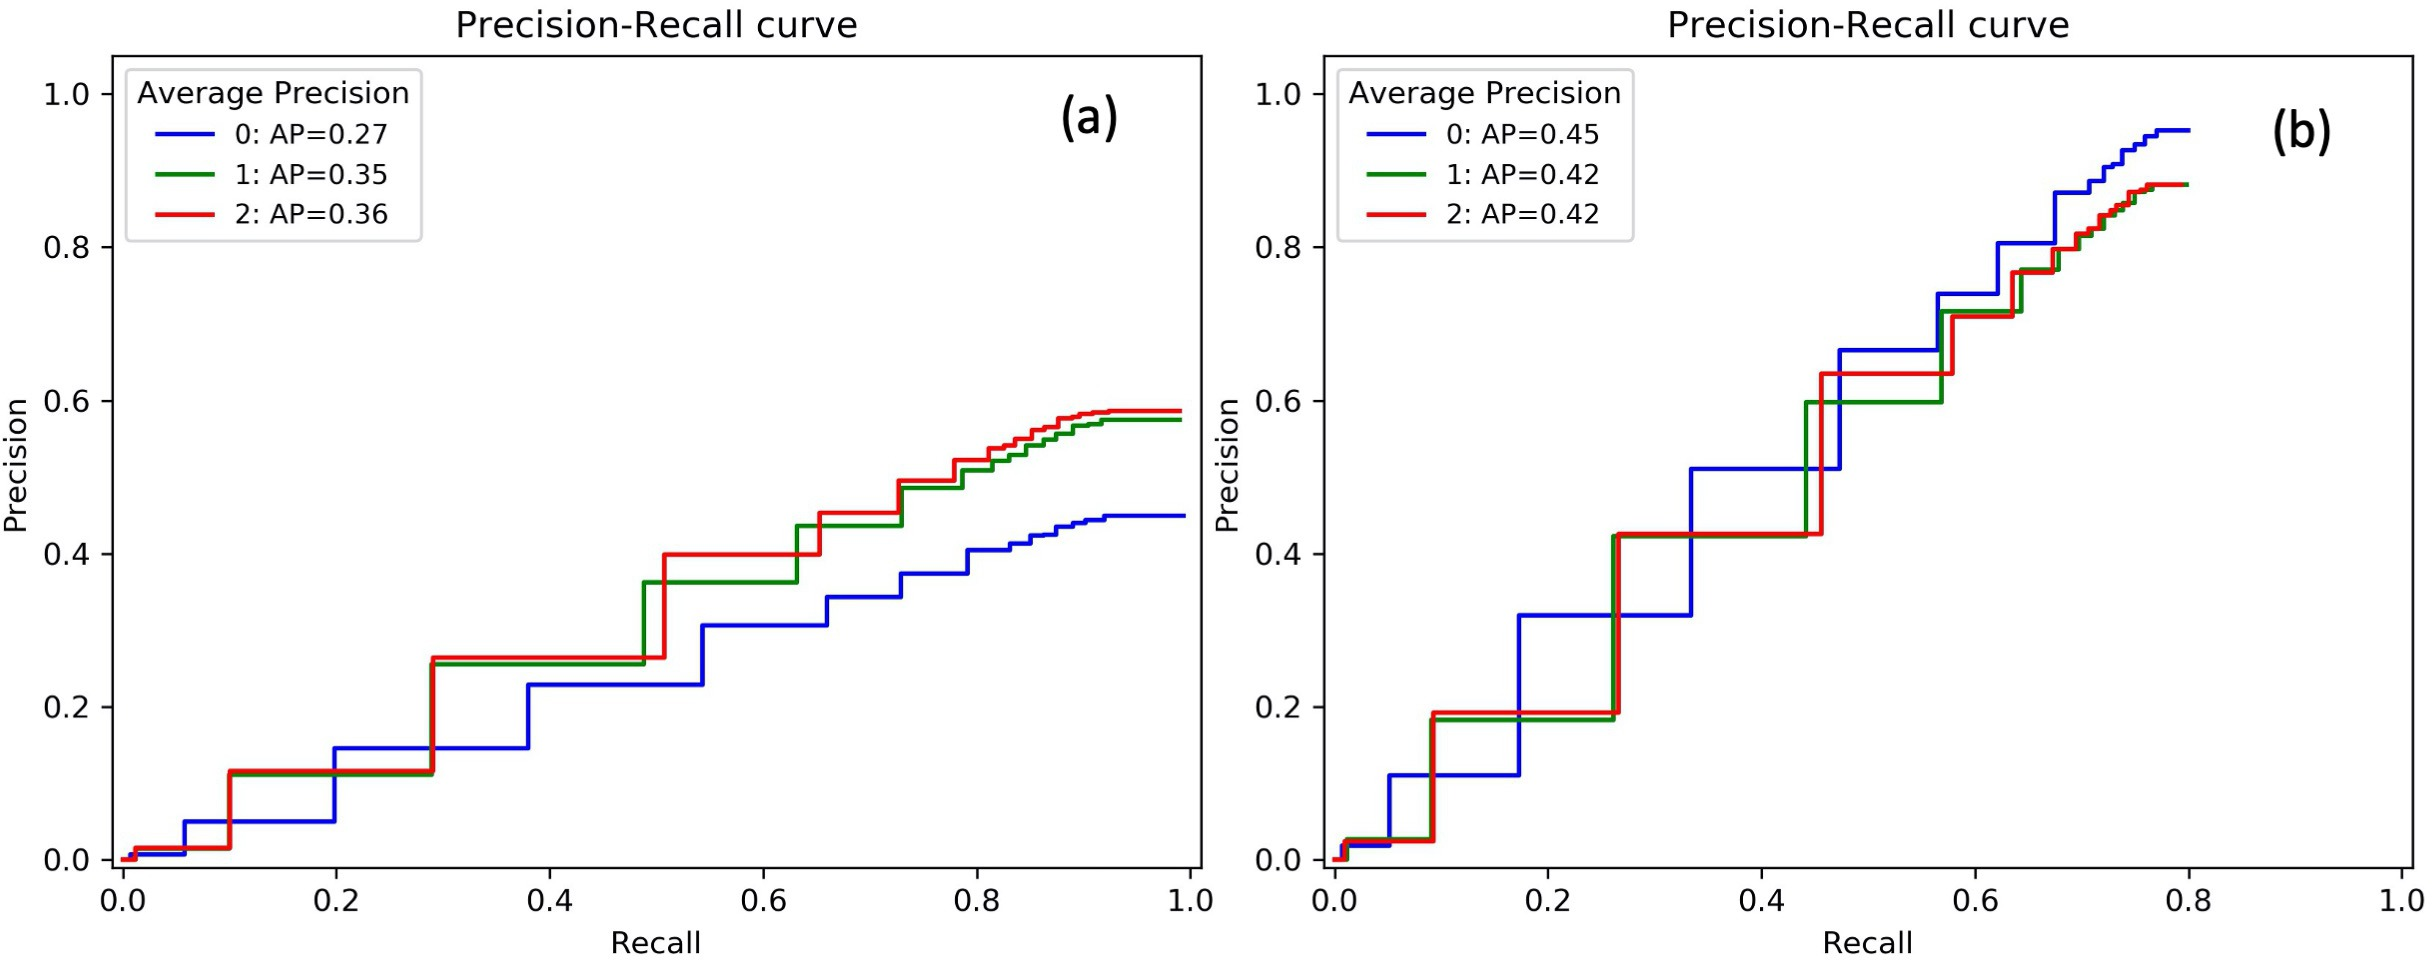
\includegraphics[width=14cm]{figs/exp14_p_r_curves_allPoly_trim.jpg}
	\caption{Precision-recall curves and average precision of mapped polygons in 2017, 2018, and 2019. (a) and (b) are precision-recall curves and AP values without and with applying the assumption of RTS dynamic features, respectively.}
	\label{fig_p_r_curve}
\end{figure}


%Table \ref{table_accuracy_f1} lists the numbers of true positives, false positives, and false negatives, as well as precision, recall, and F1 scores in each year, with and without considering RTS-dynamic features.

%Mapping results using multi-temporal remote sensing images, without negative training polygons. 
%Improvement by applying time IOU and occurrence

The F1 scores and AP values of the mapped polygons from 2017 to 2019 improve after applying the time-IOU and two-polygon assumption. 
As shown in Table \ref{table_accuracy_f1} and Fig. \ref{fig_p_r_curve}, the F1 scores improve by around 0.2, from $\sim$0.6 to $\sim$0.8, and the AP values improve from around 0.35 to around 0.45. 
By utilizing the dynamic features of RTSs in the multi-temporal images, the number of false positives reduces dramatically, from around 300 to around 30 (Table \ref{table_accuracy_f1}).
%Therefore, the F1 scores and AP values improve significantly.
However, the number of true positives reduces by around 40, resulting in the increased number of false negatives. 
%TODO: need to explain this one better by  giving an example. 
The reason is that some of the mapped polygons mismatch RTS boundaries and cannot represent the RTS development over time, leading to violation to the assumption of RTS dynamic features. 
 
%compared with the ones including negative training polygons 
The assumption of RTS dynamic features can contribute more to the improvement of mapping accuracies if we exclude negative training polygons when training the network. 
As shown in Table S3, the F1 scores improve significantly after applying the RTS dynamic features, as that the FP reduces from around 1500 to less than 200, meanwhile, the AP values (Fig. S3) improve by around 0.2 in different years. 
This is because excluding negative training polygons tends to produce more false positives but usually they cannot meet the criterion of the RTS dynamic feature.  
%The reason is that include: (1) the number of false positives reduces by around 70, but the number of true positives also reduces by around 40, resulting in an almost unchanged F1 score 
%and (2) including the negative training polygons %used in \cite{huang2020using}
% has depressed the population of false positives. 


%results from k-fold cross-validation (mention it, then put into supplementary files), no k-fold results. 

\subsubsection{Comparison with one-year snapshot results}
\label{sec_compare_with_201805_results}

Both the F1 score and AP values of the mapped polygons in this paper are slightly worse than the accuracy of one-year results presented in \cite{huang2020using}. 
Regarding the F1 scores (Table \ref{table_accuracy_f1}) after applying RTS dynamic features, the difference between the one in \cite{huang2020using} and in this paper is around 0.05, while the difference of the AP values is around 0.1.
For the results only used 2017 and 2018 images for training (Table S2) or excluding negative training polygons (Table S3), the F1 score and AP values are further smaller than the one-year results by around $\sim$0.2 and $\sim$0.15, respectively. 
One possible reason is related to the variation of features over time. 
For example, the 2018 and 2019 images (Fig. \ref{fig_multi_rts_image_studyarea}c and d) are brighter than the 2017 image (Fig. \ref{fig_multi_rts_image_studyarea}b), leading to the challenges of training the DeepLabv3+ and lowing its performance. %which may confuse the DeepLabv3+ model during training. 

%need to talk about the different between over 300 polygons and ~260 polygons. I did, in the manual delineation section.  

%Compared the precision recall curves, the AP value is smaller, because we don't have the high values of recall and precision. 


\subsection{RTS expansion from 2017 to 2019}
\label{sec_rts_expanding}

% the figure here, shows change area and retreat distance, are derived from manual delineation.
\begin{figure} 
	\centering
	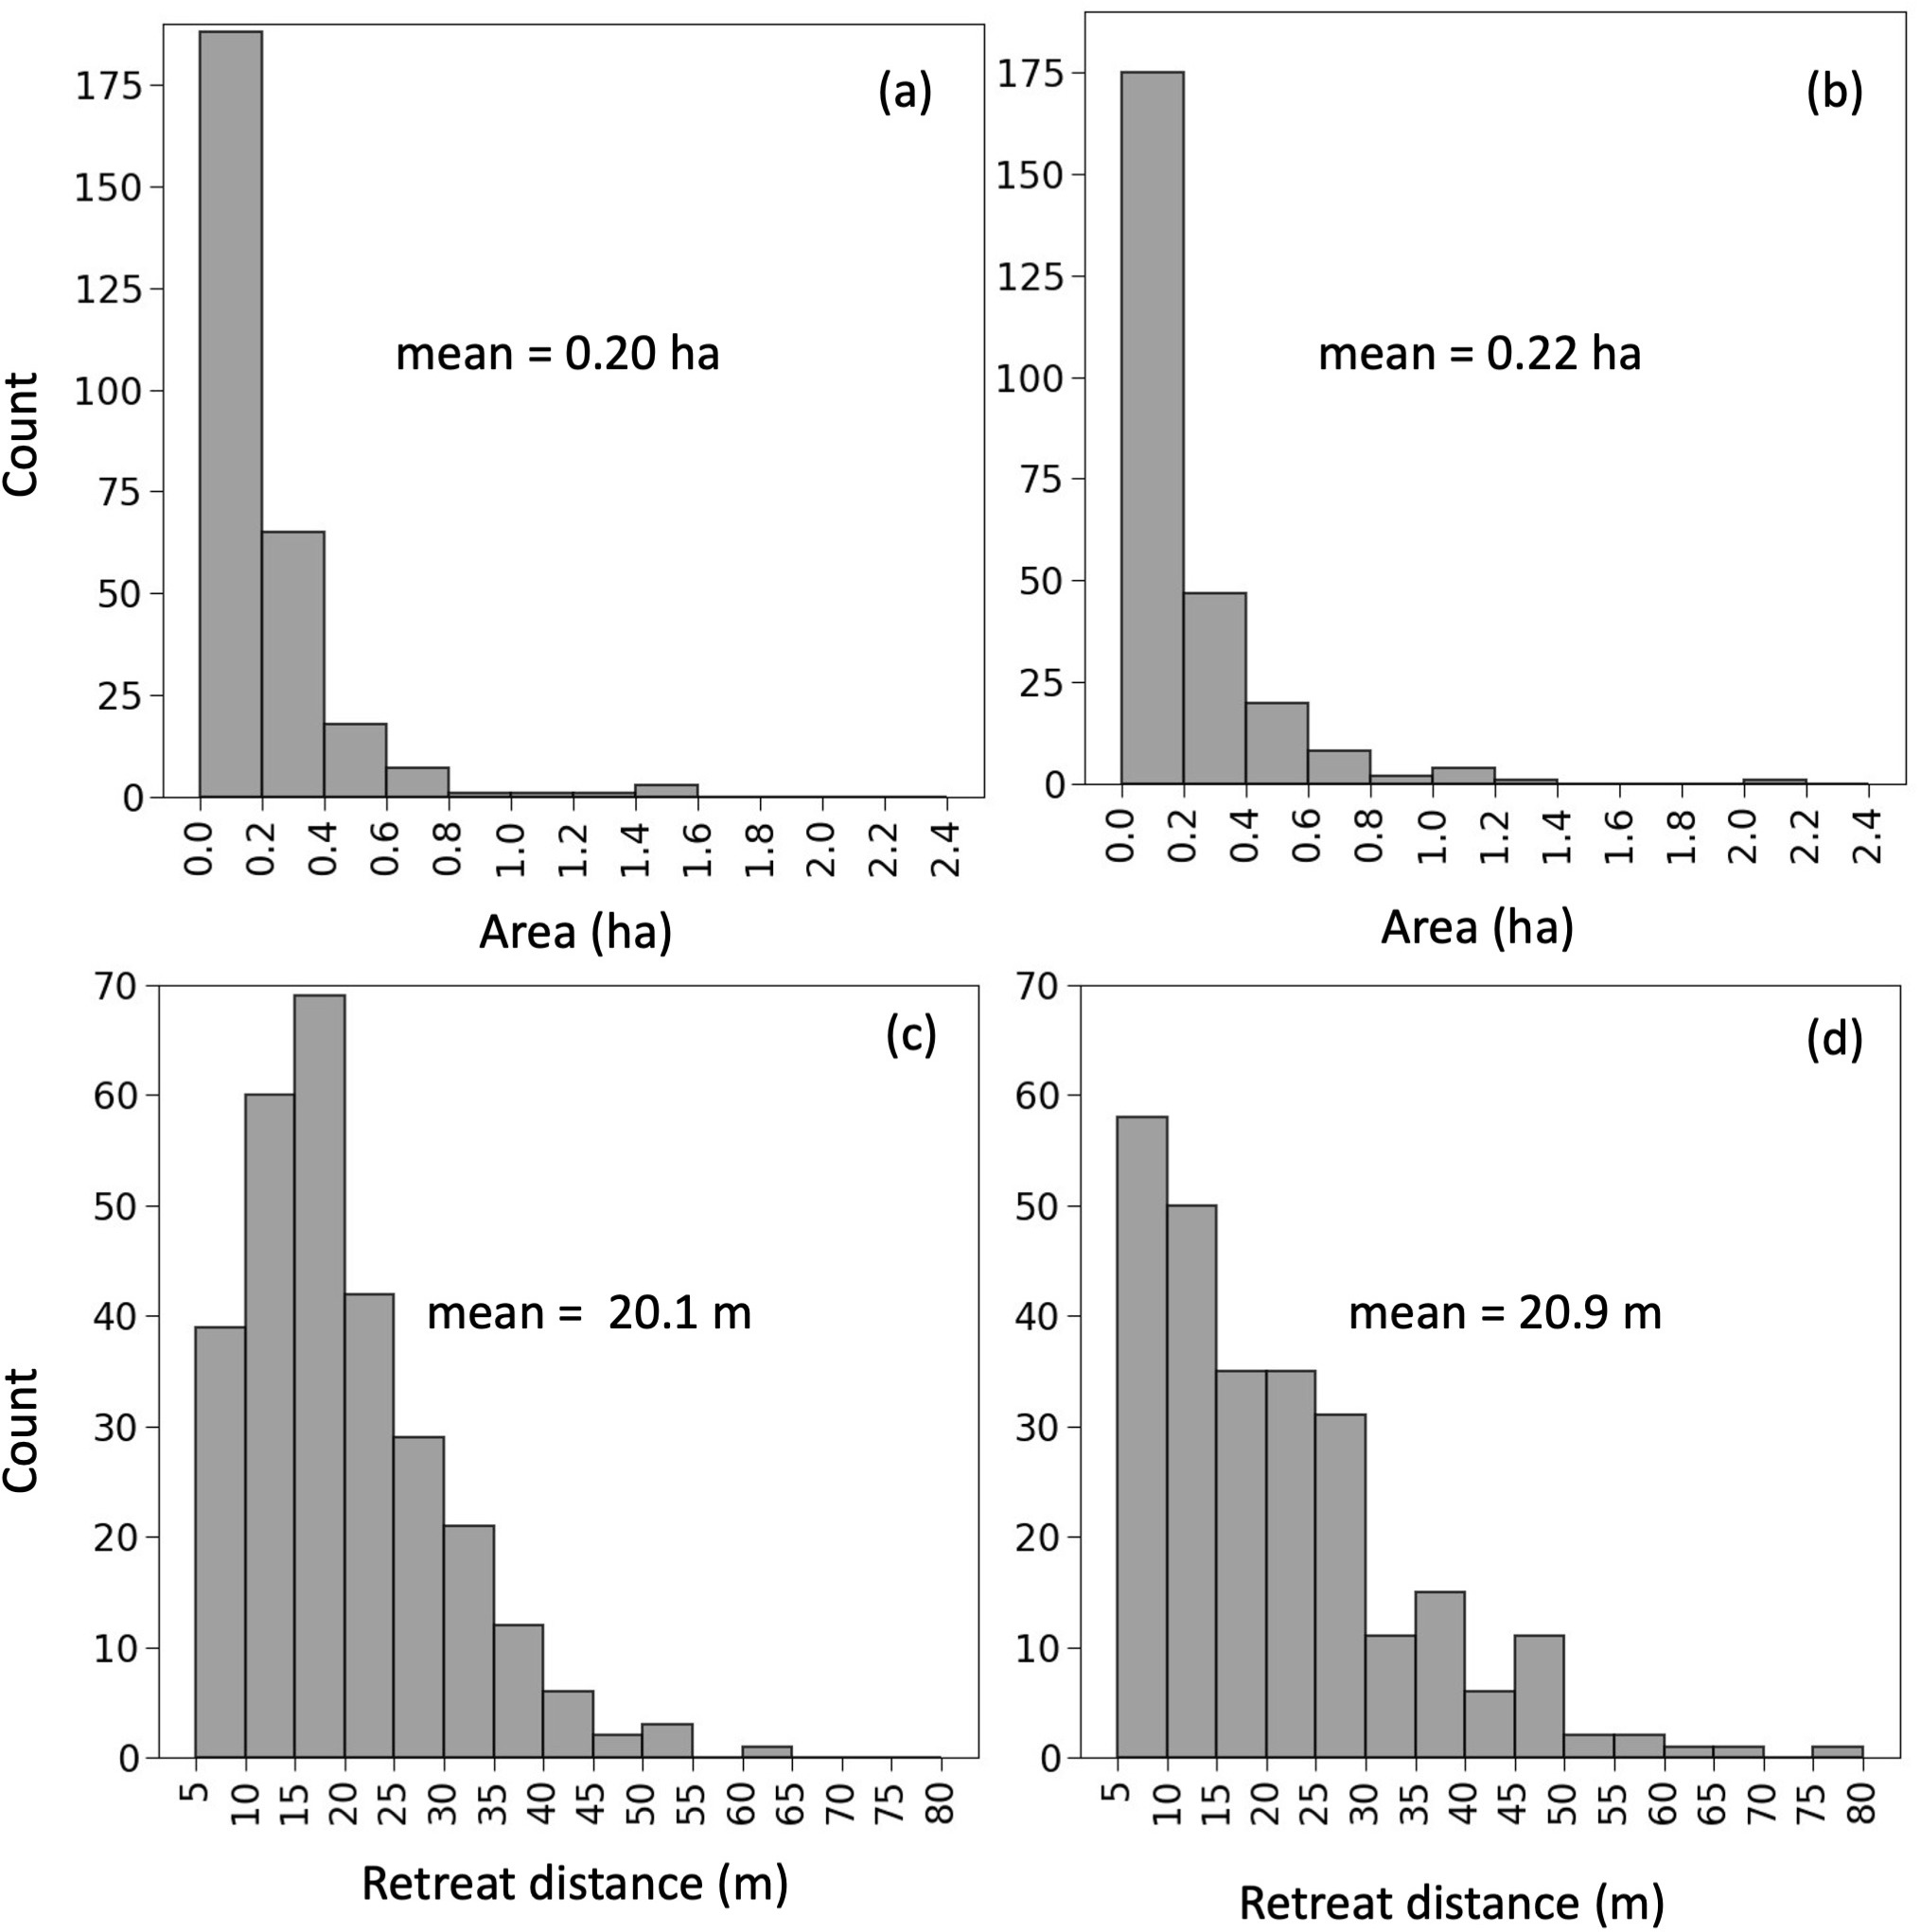
\includegraphics[width=14cm]{figs/rts_change_area_dis_manu_v2_trim.jpg}
	\caption{Histograms of RTS expansion areas and retreat distances. (a) and (b) are expanding areas of 2018 vs 2017 and 2019 vs 2018, respectively. One RTS with an expanding area of 2.53 ha is not included in (b) because it exceeds the axis range. (c) and (d) are retreat distances from 2017 to 2018 and 2018 to 2019, respectively.}
	\label{fig_rts_change_area_reDis}
\end{figure}

\subsubsection{Area of RTS expansion}
\label{sec_rts_change_area}

% In the manual delineation results, we have 266, 266, and 267 RTSs in 2017, 2018, and 2019 images, respectively. 
% In the RSE 2020 paper, we identify 263 RTSs (2018 May images).

In the Beiluhe region, most RTS expanded from 2017 to 2019 with an average expanding area of 0.20 ha from 2017 to 2018 and 0.22 ha from 2018 to 2019 as shown in Fig. \ref{fig_rts_change_area_reDis}a and b.
From 2017 to 2018, 284 RTSs expanded, among them, 96 ones with expanding area greater than 0.2 ha; while from 2018 to 2019, 259 RTSs expanded, and 84 of them expanded by greater than 0.2 ha.
The maximum expanding areas are 1.47 ha and 2.53 ha for 2017 vs 2018 and 2018 vs 2019, respectively. 
The ground truths outline 342 RTSs in Beiluhe, therefore, 83\% of them expanded from 2017 to 2018 and 76\% from 2018 to 2019. 
As shown in Fig. S4, around half of the RTSs only had one expanding branches, while each of the remaining ones (152 for 2017 vs 2018 and 117 for 2018 vs 2019)  had two or more expanding branches. 

%How to define an RTS was expanding?
%How many RTS have expanding? 
%not to define, just say how many has expanding area greater than ...?



\subsubsection{RTS retreat distance}
\label{sec_rts_retreat_distance}

%retreat distance from 2017 to 2019. 
%add standard variation for retreat distance.  done
The average retreat distances of RTSs from 2017 to 2018 and 2018 to 2019 were 20.1 m and 20.9 m (Fig. \ref{fig_rts_change_area_reDis}c and d), respectively. 
The maximum retreat distances were 61.9 m and 77.2 m for 2017 vs 2018 and 2018 vs 2019, respectively, based on medial circles. 
From 2017 to 2018, 65\% of RTSs retreated more than 15 m, while from 2018 to 2019, 58\% of them had retreat distance greater than 15 m. 
% measure the retreat distance from manual delineation, mentioned here or in the (discussion) supplementary materials?
%show planet images in different years for this one
In Fig. S5, the mean retreat distances based on the manually drawn lines are 21.3 m and 25.0 m for 2017 vs 2018 and 2018 vs 2019, respectively, while the maximum retreat distances were 90.8 m and 212.8 m (Fig. \ref{fig_rts_example1}).


 % standard deviation
\begin{figure} 
	\centering
	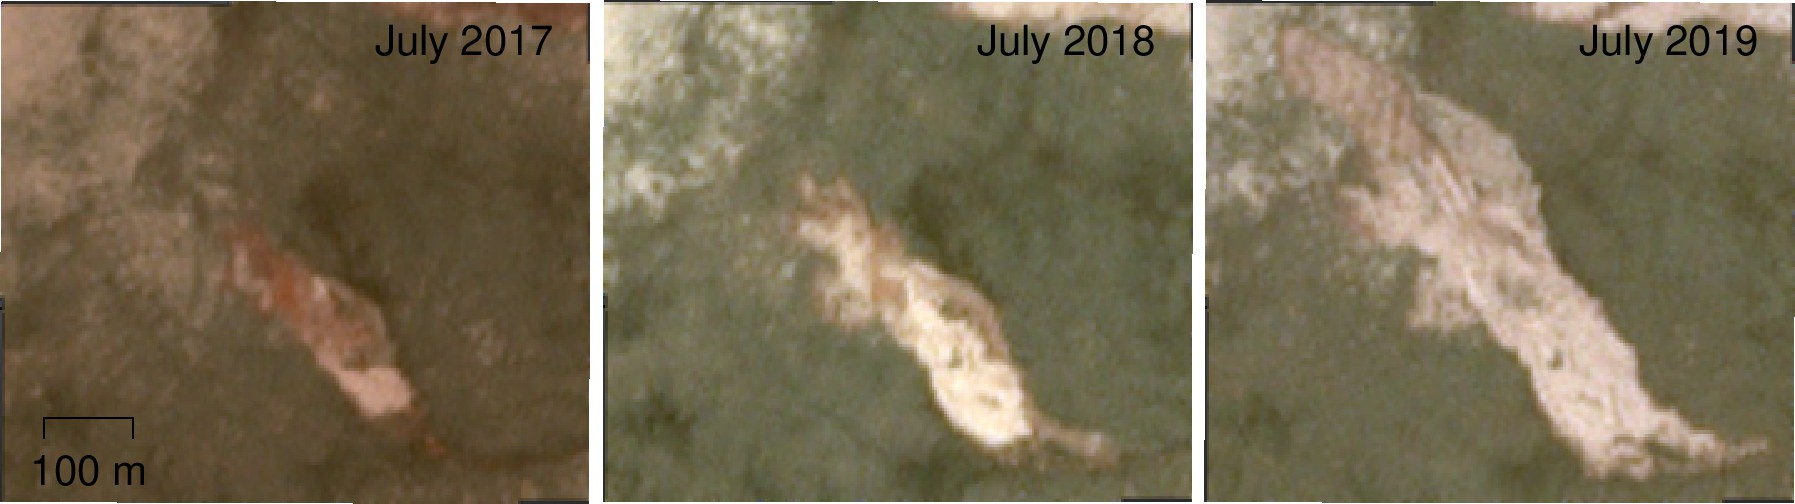
\includegraphics[width=14cm]{figs/img_2017_to_2019_ex1.jpg}
	\caption{Planet images of the RTS (92.580$^\circ$ E, 34.969$^\circ$ N) with the maximum retreat distance among all the mapped ones in the study area. Its headwall retreated by 212 m from 2018 to 2019.}
	\label{fig_rts_example1}
\end{figure}


%Other measurement,  uncertainty, and standard variation
The three automatic measurements of retreat distances are slightly different from the ones derived from manually drawn lines. Among them, the one based on the diameter of the maximum medial circle is closest to the manual measurement. 
As shown in Fig. S6, the mean differences are $-1.3$ m \& $-4.1$ m, 17.9 m \& 14.4 m (2017 vs 2018 \& 2018 vs 2019), and 13.4 m \&9.7 m for the one based on the diameter of the maximum medical circles, the direction of the maximum elevation difference, and across the centroid of old polygons, respectively. 
%Retreat distance estimated based on diameter of the maximum medical circles tends to be underestimated but a few one them 
As mentioned in section \ref{sec_cal_retreat_dis}, the retreat distance calculated from medial circles tend to be underestimated due to the nature of inscribed circles, but the other two automatic measurements are overestimated. 
There are also some special cases that the retreat distance of some RTSs based on medial circles are greater than the one from manually draw lines as shown in the histogram (Fig. S6).
The reason is that the manually drawn lines may not exactly match the direction of the maximum retreat.  

 % standard deviation
\begin{figure} 
	\centering
	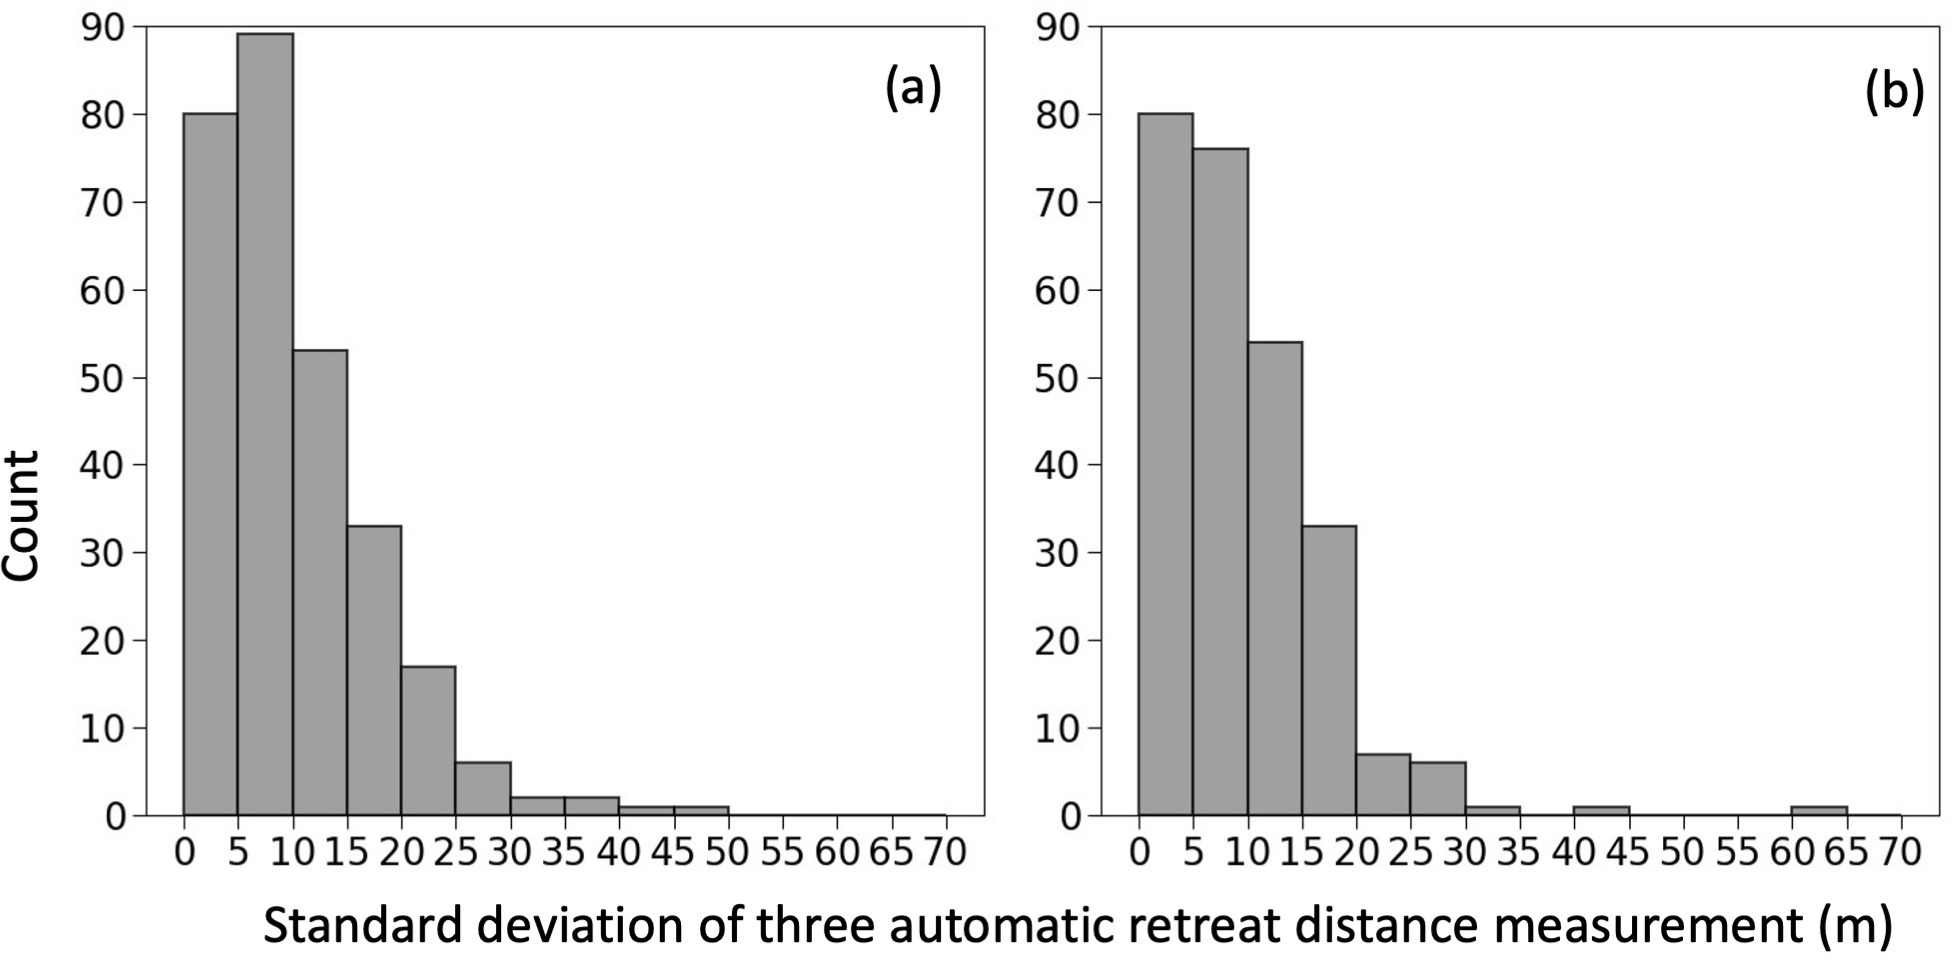
\includegraphics[width=14cm]{figs/standard_deviation_v2_trim.jpg}
	\caption{Histograms of the standard deviations of three automatic retreat distance measurements. (a) shows the standard deviations for 2017 vs 2018, and (b) for the ones of 2018 vs 2019, respectively.}
	\label{fig_re_dis_standard_var}
\end{figure}

% why you think 30 can be used to defined a good agreement? need to think more, such as their difference? within the delineation errors?
% has change 30 to 10 m
The retreat distances of most RTSs measured by the three automatic methods are consistent as represented by the standard deviations (Fig. \ref{fig_re_dis_standard_var}).
From 2017 to 2018, the percentage of RTSs have standard deviations smaller than 10 m is 60\%, while for 2018 to 2019, it is 59\%, demonstrating a good agreement among the three measurements.
However, standard deviations of around 40\% of them are quite large ($>$10 m), indicating the complex and irregular shapes of the change polygons. 
 


% compare with other retreat distance reported in other region?  in discussion session.   no need. 
 

% compare the retreat rates derived from automatic results and manual delineation. 
% have shown a brief comparison.

\subsubsection{RTS expansion based on automatic delineation}
\label{sec_rts_change_auto_mapping}

As shown in Fig. S7, the average values of expanding areas and retreat distances of RTS boundaries derived based on automatic delineation are similar to the one from manual delineation (section \ref{sec_rts_change_area} and \ref{sec_rts_retreat_distance}).
In Fig. S7, the average expanding areas are 0.25 ha (2018 vs 2017) and 0.24 ha (2019 vs 2018), and the mean retreat distances are 21.5 m (2018 vs 2017)  and 21.6 m (2019 vs 2018). 
However, the total number of expanding RTSs is smaller at 236 (2018 vs 2017) and 233 (2019 vs 2018), respectively, due to the false negatives in the automatic delineation results.

 

\section{Discussion}
\label{sec_discussion}

%\subsection{Advantage and disadvantage of using the RTS dynamic feature}
%\label{sec_diss_rts_dynamic_features}
%\subsection{Delineating RTS boundaries on multi-temporal images}
\subsection{Advantages and limitations of automatic delineation}
\label{sec_diss_mapping_rts_multi_images}

The deep-learning-based method can automatically delineate RTS boundaries on multi-temporal images with high accuracies and can potentially be applied to large areas to investigate RTS development. 
As demonstrated in this paper, the results from the automatic method can accurately delineate most RTS boundaries in different years.
%Accurate RTS boundaries from multi-temporal images are essential for quantifying their development.
Based on these multi-temporal boundaries, we can reveal their development in unprecedented spatial and temporal details. 
Although automatic delineation misses some RTSs and produces many inaccurate boundaries, based on its results we still can obtain similar values of RTS development (section \ref{sec_rts_change_auto_mapping}). 


However, to delineate RTS boundaries on multi-temporal images is more challenging than to identify their location or on one-year images. 
In this study, the targets are not only locations and extents of 342 RTSs in Beiluhe, but also their boundaries in different years, that is, $342\times3$ RTS boundaries from 2017 to 2019.
As shown in section \ref{sec_compare_with_201805_results}, the F1 scores derived from multi-temporal images are slightly worse than one-year results, indicating the challenges of mapping RTSs in multi-temporal images. 
The possible reasons include (1) the inconsistent features of the same RTS in different images may lower the performance of the trained model 
and (2) inaccurately mapped boundaries cannot meet the requirement of RTS dynamic features. 
These reasons are related to the mapping strategy, that is, training a single model and removing false mapped polygons by applying RTS dynamic features.  
Alternatively, we may adopt other strategies such as training multiple models, one model for each year,  which is still manageable when images only span a few years.
Applying the RTS dynamic feature can significantly reduce the number of false positives (section \ref{sec_improve_using_multi_images}), but it also removes some correctly mapped polygons with relatively lower delineation accuracy. 
%Lowering the criteria of RTS dynamic features can help identify more mapped polygons but also reserved more RTS   %or adding some negative training polygons for training if they are available.
Another limitation of applying the RTS dynamic features is that a new emergent RTS (in or after 2019) would be removed. 


%Advantage: do not need negative training polygons, so save time when extend to larger areas.

\subsection{Advantages and limitations of automatic calculation of retreat distance}
\label{sec_diss_retreat_distance}

Automatic calculation of RTS retreat distance is necessary for investigating RTS development in large areas.
Currently, measurement of RTS retreat distance is conducted in the field or on images using manual measurement, which is limited to local areas. 
In this study, a proposed method based on polygon-based change detection and medical circles fills the gap of the automatic calculation of RTS retreat distance 
and provides an effective tool for quantifying RTS development in large areas. 
Moreover, the input polygons (RTS boundaries) can be either derived from manual delineation or automatic mapping methods, 
providing the ability and flexibility to utilize both archived and newly produced data.


The retreat distance of most RTSs are equal or close to manual measurement on images, and only a few of them show large discrepancies due to irregular or elongated shapes of expanding areas. 
%Why we need three automatic measurement for the retreat distance?
Therefore, in addition to the automatic measurement of medical circles, we also conduct two other automatic measurements (based on DEM difference and centroid of the corresponding old polygon) as supplementary measurements. 
For a specific RTS, further investigations are needed if the discrepancy (represented by standard deviation) is large. 
These irregular or elongated shapes of expanding areas may cause by the spatial distribution of ground ice and micro-terrain.
The accuracy of RTS boundaries (input polygons) can affect the accuracy of retreat distance, especially when these boundaries are derived from automatic mapping methods. 
Currently, automatic mapping (multi-temporal or one-year) usually produces a few mapped polygons that are inaccurate, leading to the uncertainties of retreat distance. 
Therefore, in the future, we may consider using pixel-based change detection to obtain the expanding area directly from multi-temporal images. 



%\subsection{Comparison with RTS retreat rates in the Arctic}
%
%No report of RTS retreat in the Tibetan Plateau, but the one in the Arctic.


\section{Conclusions}
\label{sec_conclusion}

We proposed a method based on DeepLabv3+, change detection, and medial axis transform to automatically quantify the development of retrogressive thaw slumps in the Beiluhe region. 
Experiments show that the results from the automatic delineation of RTS boundaries on multi-temporal images are close to the one from manual delineation for most RTSs, indicating the good performance of DeepLabv3+  that not only for identifying their locations but also for accurately delineating their boundaries. 
However, the results also indicate the challenge of automatic delineation when applying DeepLabv3+ to multi-temporal images when compared with one-year results. 
With the input of multi-temporal RTS boundaries, either from automatic or manual delineation, our method can obtain their expanding regions, then further produce their change areas and retreat distances based on medial circles. 
The whole process is automatic and can be used an effective and efficient tool for quantifying RTS development in large areas. 

Most of the RTSs in the Beiluhe region were expanding from 2017 to 2019 with significant expanding areas and retreat distances. 
Among the 342 RTSs, 83\% of them expanded from 2017 to 2018 and 76\% from 2018 to 2019, with an average expanding area of 0.20 ha and 0.22 ha, respectively.
The average retreat distances of RTSs were 21.3 m (2017 vs 2018) and 25.0 m (2018 vs 2019).
This is the first report of RTSs retreat distance and expanding areas on the Tibetan Plateau and provides valuable information for understanding permafrost degradation in this region. 


\section{Data and codes}
\label{sec_data_codes}

Planet images can be downloaded via \url{https://www.planet.com}. 
The multi-temporal RTS boundaries will be provided by L. Huang upon request. 
%TODO: need to remove acceptance after publish. 
Codes are available on GitHub (\url{https://github.com/yghlc/ChangeDet_DL}) after the acceptance of this paper.

\section{Acknowledgments}
\label{sec_acknowledgments}

%TODO: thanks editors reviewers after review

Thanks to Planet's Education and Research Program, through which we downloaded CubeSat images for this study. 
%Thanks to Drs. Jing Luo, Zhanju Lin, and Fujun Niu at Northwest Institute of Eco-Environment and Resources, Chinese Academy of Sciences for their support and arrangement of the Beiluhe field work in 2018. 
This work is funded by the Hong Kong Research Grants Council (CUHK14303119).


%% The Appendices part is started with the command \appendix;
%% appendix sections are then done as normal sections
%% \appendix

%% \section{}
%% \label{}

\section{References}
\label{sec_reference}

%% If you have bibdatabase file and want bibtex to generate the
%% bibitems, please use
%%
\bibliographystyle{elsarticle-harv} 
%\bibliography{polygon_based_rts_changeDet.bib}
% the bib file in "~/codes/Texpad/shared_files"
\bibliography{permafrost_rs_ref.bib}

%% else use the following coding to input the bibitems directly in the
%% TeX file.

%\begin{thebibliography}{00}
%
%%% \bibitem[Author(year)]{label}
%%% Text of bibliographic item
%
%\bibitem[ ()]{}
%\end{thebibliography}


\end{document}

\endinput
%%
%% End of file `elsarticle-template-harv.tex'.
